\documentclass [aspectratio=169]{beamer}
\beamertemplatenavigationsymbolsempty
\usetheme{Boadilla}
\usepackage{textpos} % package for the positioning
\usepackage[]{graphicx}
\usepackage{graphicx}
\usepackage{float}
\usepackage{hyperref}
\usepackage{caption}
\usepackage{subcaption}
\usepackage{algorithm,algpseudocode}
\usepackage[export]{adjustbox}
\usepackage{tikz}
\usepackage[square,numbers]{natbib}
\usepackage[byname]{smartref}
\usetikzlibrary{positioning}
\usetikzlibrary{arrows, shapes, decorations, automata, backgrounds, fit, petri, calc}

\newcommand*{\logofont}{\fontfamily{phv}\selectfont}

\definecolor{uwopurple}{RGB}{79,38,131} % official purple color for uwo

\title[]{\vspace{60pt} \\
Xenon} % Change the lecture topic right here!
%\subtitle{n}
\author[]{J.J. Gómez Cadenas}
\institute[]{Donostia International Physics Center}
\date{\today}

% Math notations
\newtheorem{thm}{Theorem}[section]
\newtheorem{lem}[thm]{Lemma}

\newtheorem{defn}[thm]{Definition}
\newtheorem{eg}[thm]{Example}
\newtheorem{ex}[thm]{Exercise}
\newtheorem{conj}[thm]{Conjecture}
\newtheorem{cor}[thm]{Corollary}
\newtheorem{claim}[thm]{Claim}
\newtheorem{rmk}[thm]{Remark}

\newcommand{\ie}{\emph{i.e.} }
\newcommand{\cf}{\emph{cf.} }
\newcommand{\into}{\hookrightarrow}
\newcommand{\dirac}{\slashed{\partial}}
\newcommand{\bbonu}{\ensuremath{\beta\beta0\nu}}
\newcommand{\bbtnu}{\ensuremath{\beta\beta2\nu}}
\newcommand{\mbb}{\ensuremath{m_{\beta\beta}}}
\newcommand{\qbb}{\ensuremath{Q_{\beta\beta}}}
\newcommand{\mbbsq}{\ensuremath{m_{\beta\beta}^2}}
\newcommand{\tonu}{\ensuremath{(T_{1/2}^{0\nu})^{-1}}}
\newcommand{\gonu}{\ensuremath{G^{0\nu}}}
\newcommand{\monu}{\ensuremath{| M^{0\nu}|^2}}
\newcommand{\XE}{\ensuremath{{}^{136}{\rm Xe}}}
\newcommand{\GE}{\ensuremath{{}^{76}{\rm Ge}}}
\newcommand{\TE}{\ensuremath{{}^{130}{\rm Te}}}
\newcommand{\MO}{\ensuremath{{}^{100}{\rm Mo}}}
\newcommand{\nne}{\ensuremath{\bar{N}_e}}
\newcommand{\nng}{\ensuremath{\bar{N}_\gamma}}
\newcommand{\so}{\ensuremath{\rm S_1}}
\newcommand{\st}{\ensuremath{\rm S_2}}
\newcommand{\tz}{\ensuremath{\rm t_0}}
\newcommand{\R}{\mathbb{R}}
\newcommand{\C}{\mathbb{C}}
\newcommand{\Z}{\mathbb{Z}}
\newcommand{\N}{\mathbb{N}}
\newcommand{\Q}{\mathbb{Q}}
\newcommand{\LieT}{\mathfrak{t}}
\newcommand{\T}{\mathbb{T}}
\newcommand{\A}{\mathds{A}}
\newcommand{\E}{\mathbb{E}}
\newcommand{\Prob}{\mathbb{P}}
\newcommand{\Var}{\text{Var}}
\newcommand\equalhat{%
\let\savearraystretch\arraystretch
\renewcommand\arraystretch{0.3}
\begin{array}{c}
\stretchto{
    \scalerel*[\widthof{=}]{\wedge}
    {\rule{1ex}{3ex}}%
}{0.5ex}\\ 
=%
\end{array}
\let\arraystretch\savearraystretch
}

% set color
\setbeamercolor{title in head/foot}{bg=white}
\setbeamercolor{author in head/foot}{bg=white}
\setbeamercolor{date in head/foot}{fg=uwopurple}
\setbeamercolor{date in head/foot}{bg=white}
\setbeamercolor{title}{fg=uwopurple}
\setbeamerfont{title}{series=\bfseries}
\setbeamercolor{frametitle}{fg=uwopurple}
\setbeamerfont{frametitle}{series=\bfseries}
\setbeamercolor{block title}{bg=uwopurple!30,fg=black}
\setbeamercolor{item}{fg=uwopurple}
\setbeamercolor{caption name}{fg=uwopurple!70!}


% set logo at non-title pages
%\logo{
\includegraphics[height=0.9cm]{dipc.png}\vspace*{-.45\paperheight}\hspace*{.50\paperwidth}}

\begin{document}

{
\setbeamertemplate{logo}{}
\begin{frame}
    \titlepage
    \begin{textblock*}{4cm}(0.5cm,-7.3cm)
        
\includegraphics[width=4cm]{dipc.png}
    \end{textblock*}
    \begin{textblock*}{8cm}(5.0cm,-7.0cm)
        \huge \color{uwopurple}{$\Bigr\rvert$ \hspace{0.15cm} \textbf{Lecture 2}} % Change the lecture # right here! 
    \end{textblock*}
\end{frame}
}

\begin{frame}{}
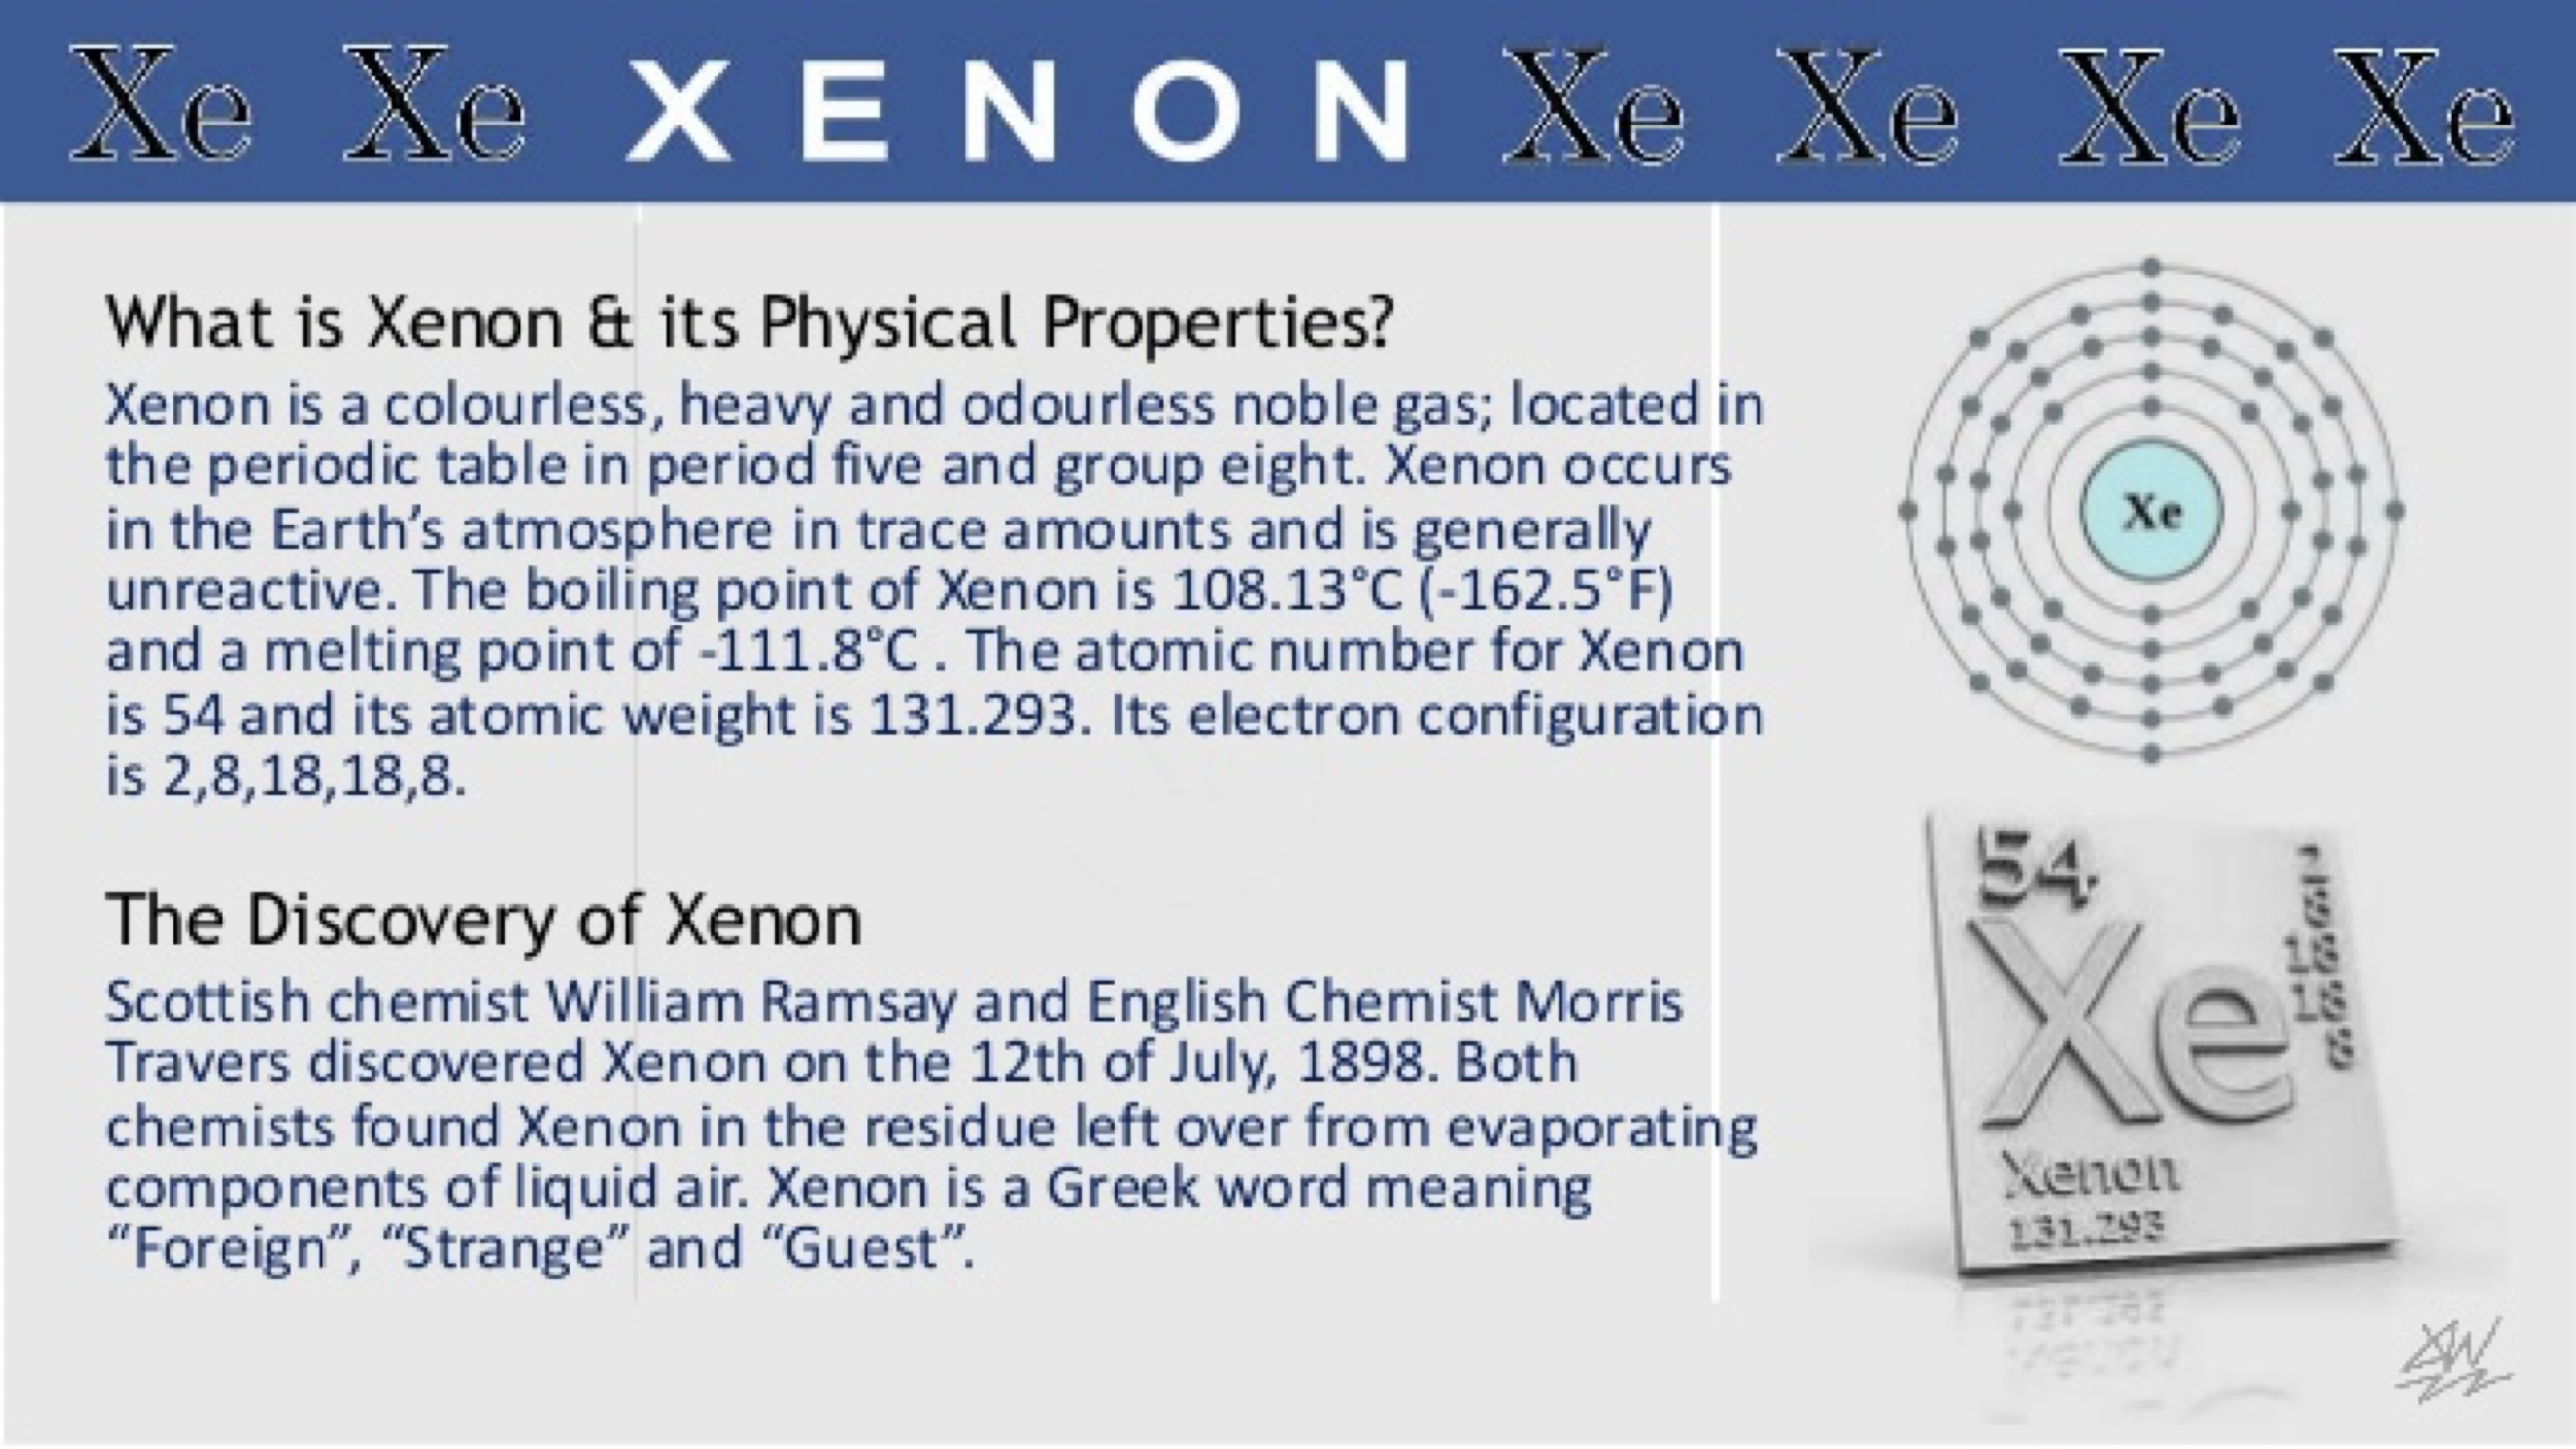
\includegraphics[scale=0.28]{ xenon1.png}
\end{frame}

\begin{frame}{}
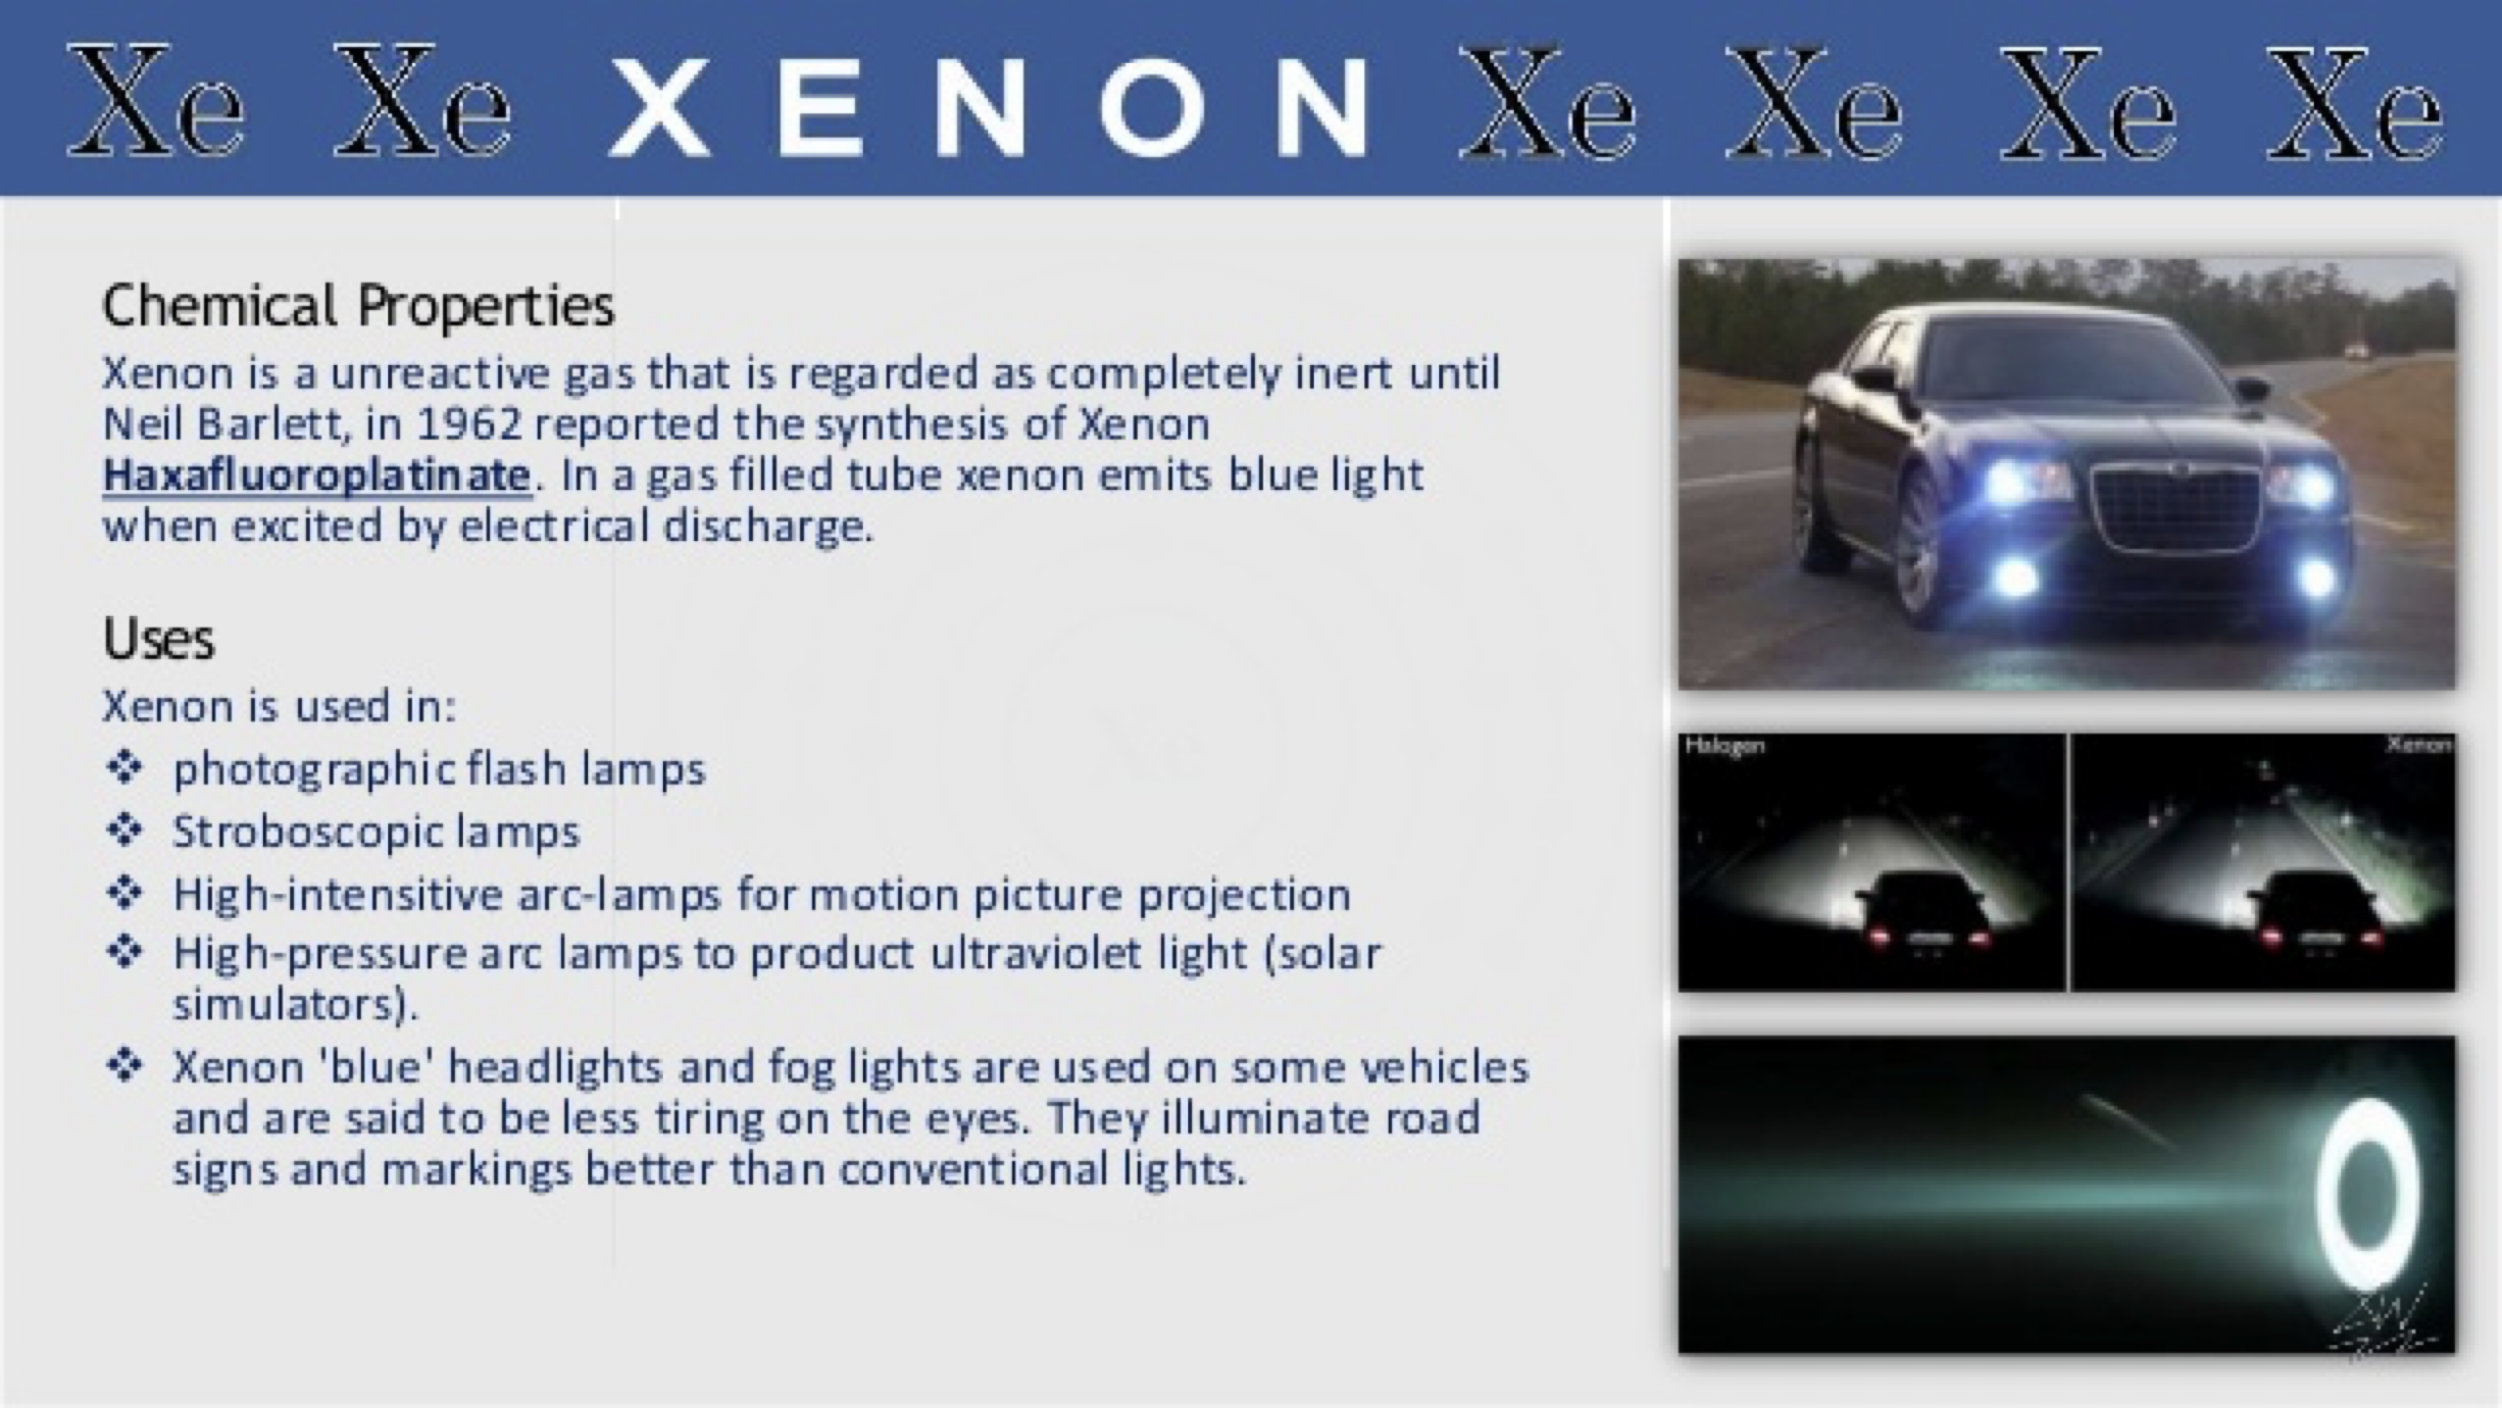
\includegraphics[scale=0.28]{ xenon2.png}
\end{frame}

\begin{frame}{Xenon Production}
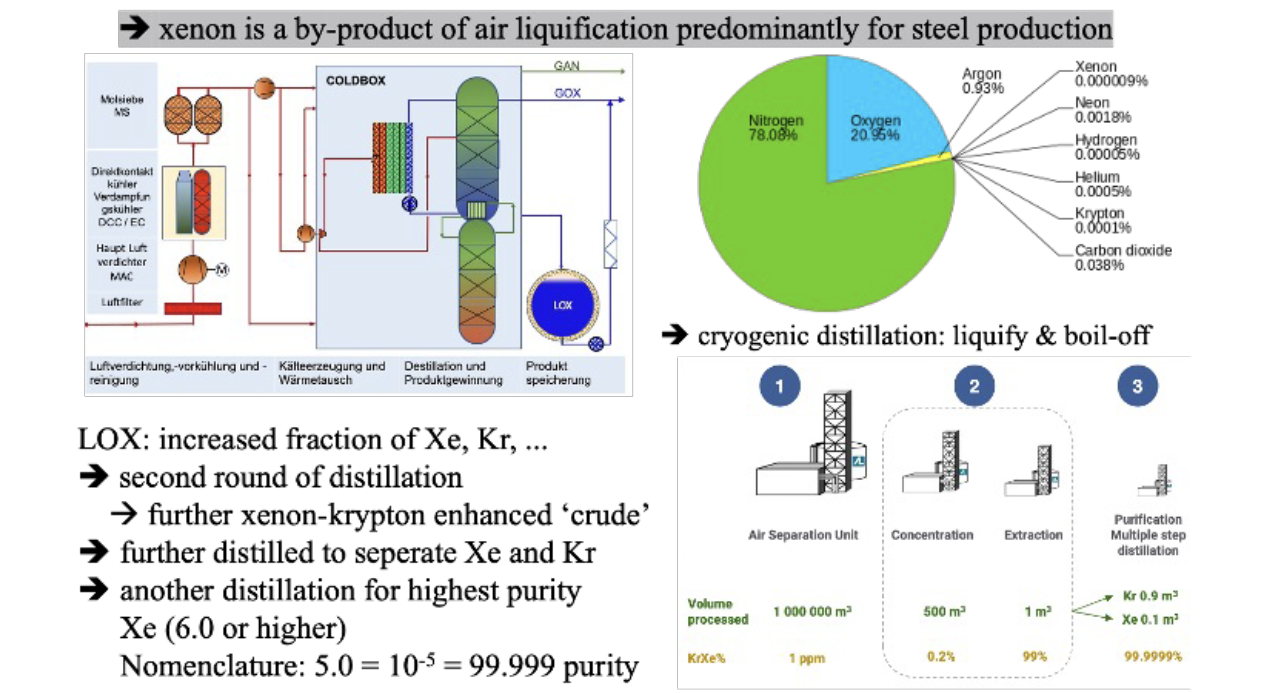
\includegraphics[scale=0.30]{xenonprod.png}
\end{frame}

\begin{frame}{Xenon Production Bottlenecks}
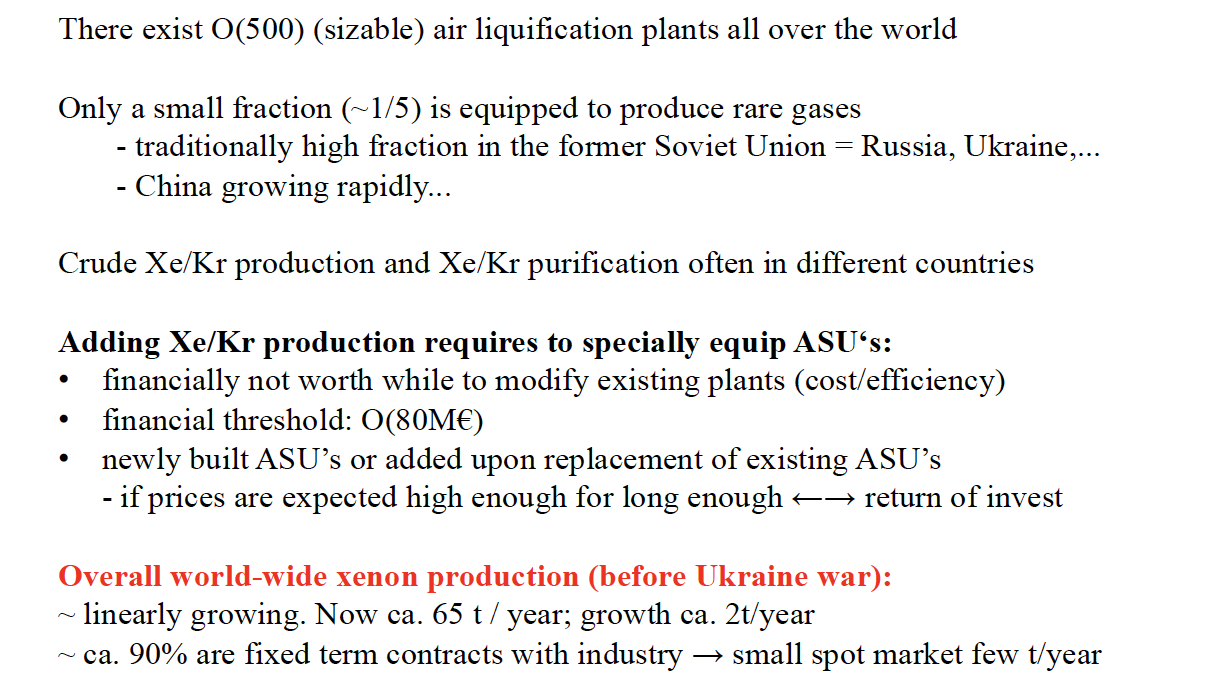
\includegraphics[scale=0.30]{xenonbottle.png}
\end{frame}

\begin{frame}{Xenon Production by Country}
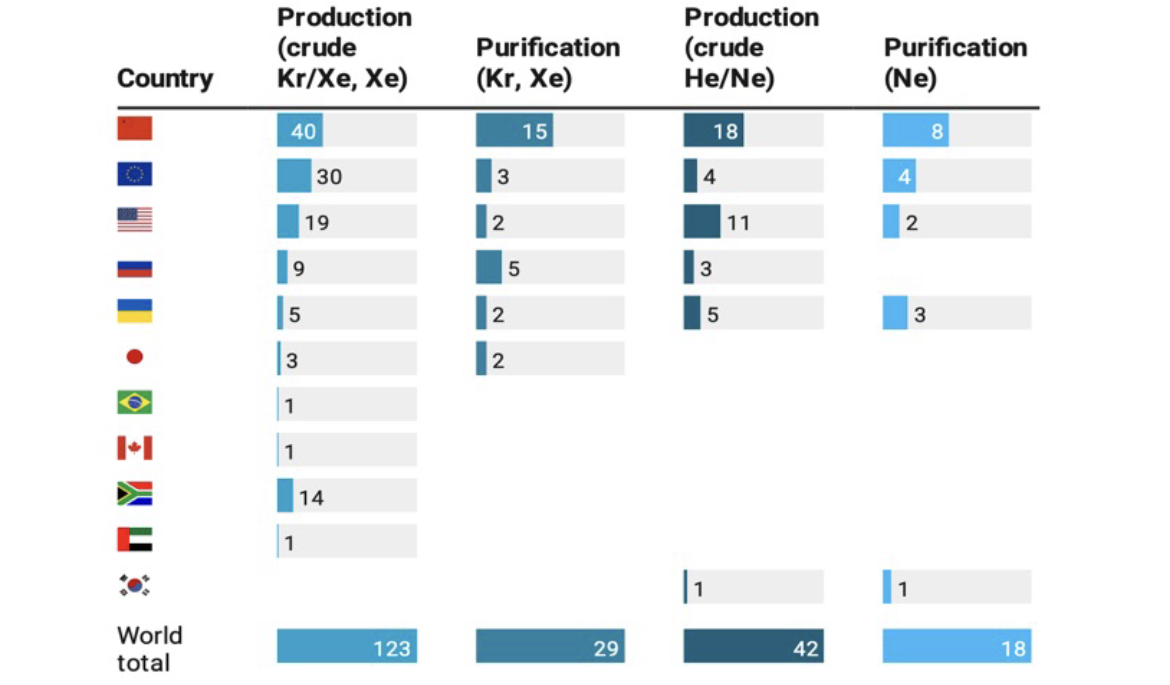
\includegraphics[scale=0.30]{asus.png}
\end{frame}

\begin{frame}{Xenon from Russia and Ukraine}
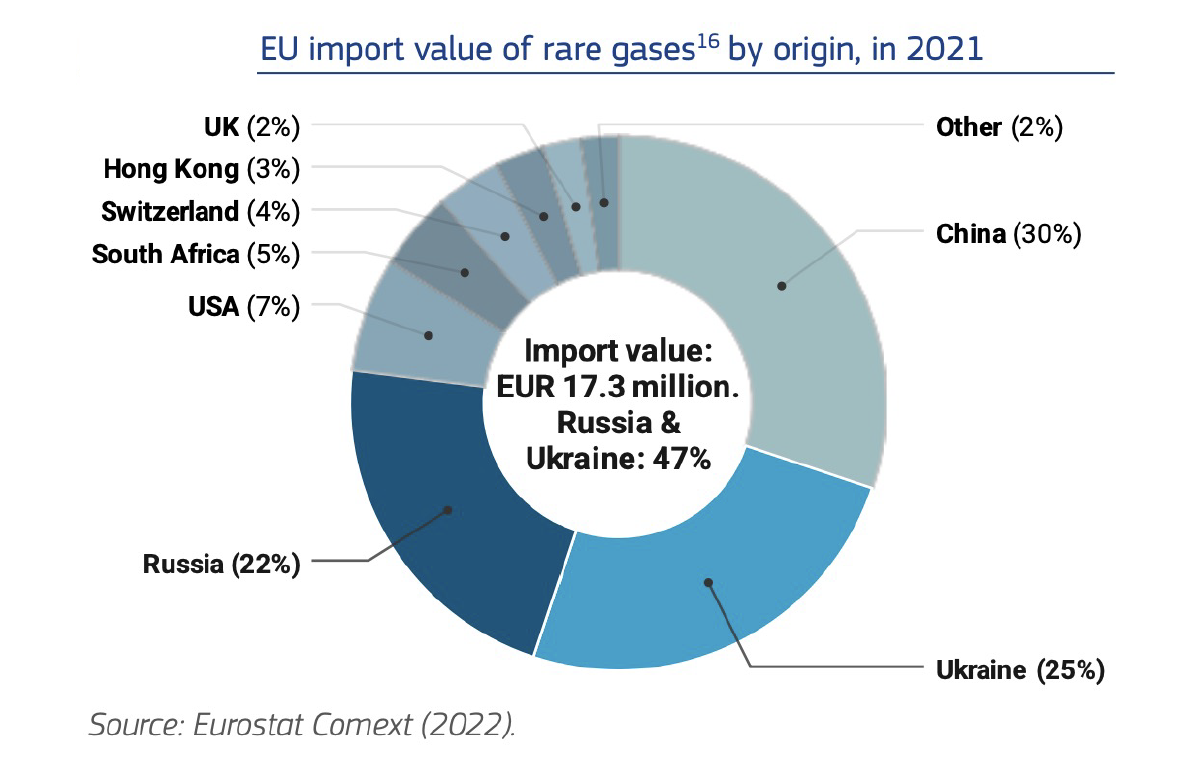
\includegraphics[scale=0.30]{gasFromRussia.png}
\end{frame}

\begin{frame}{It's the economy stupid}
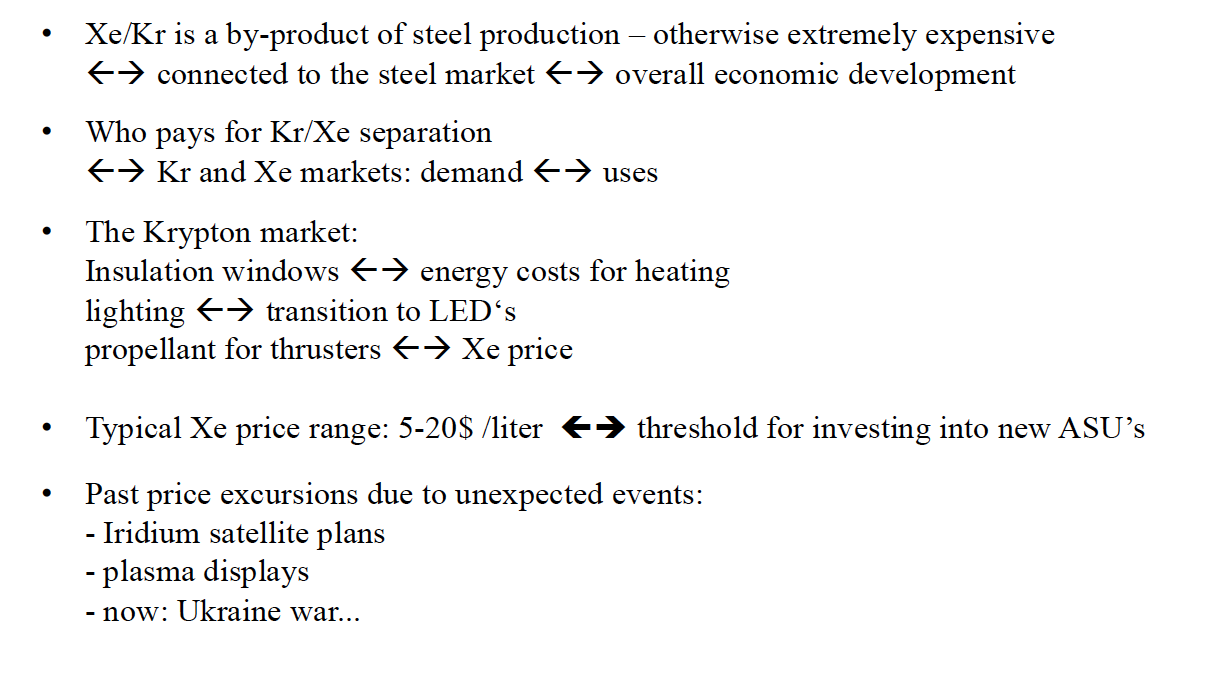
\includegraphics[scale=0.30]{commercialxe.png}
\end{frame}

\begin{frame}{A Volatile Market}
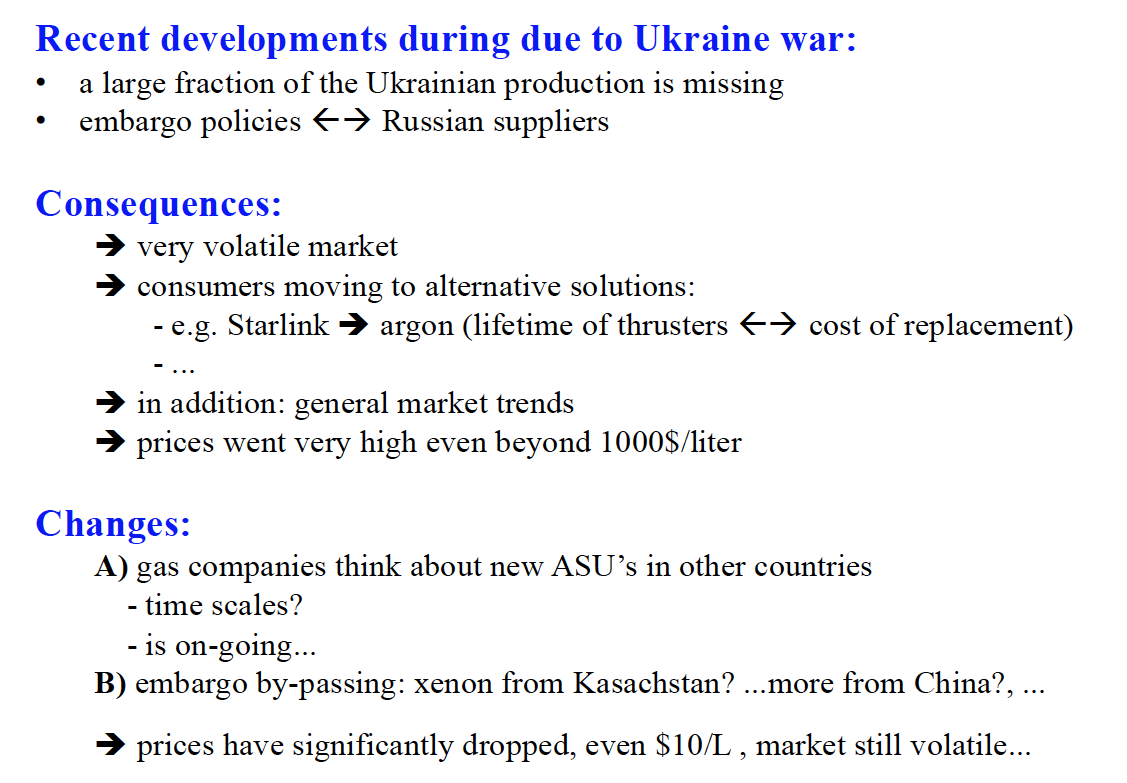
\includegraphics[scale=0.25]{volatile.png}
\end{frame}

\begin{frame}{A Volatile Market}
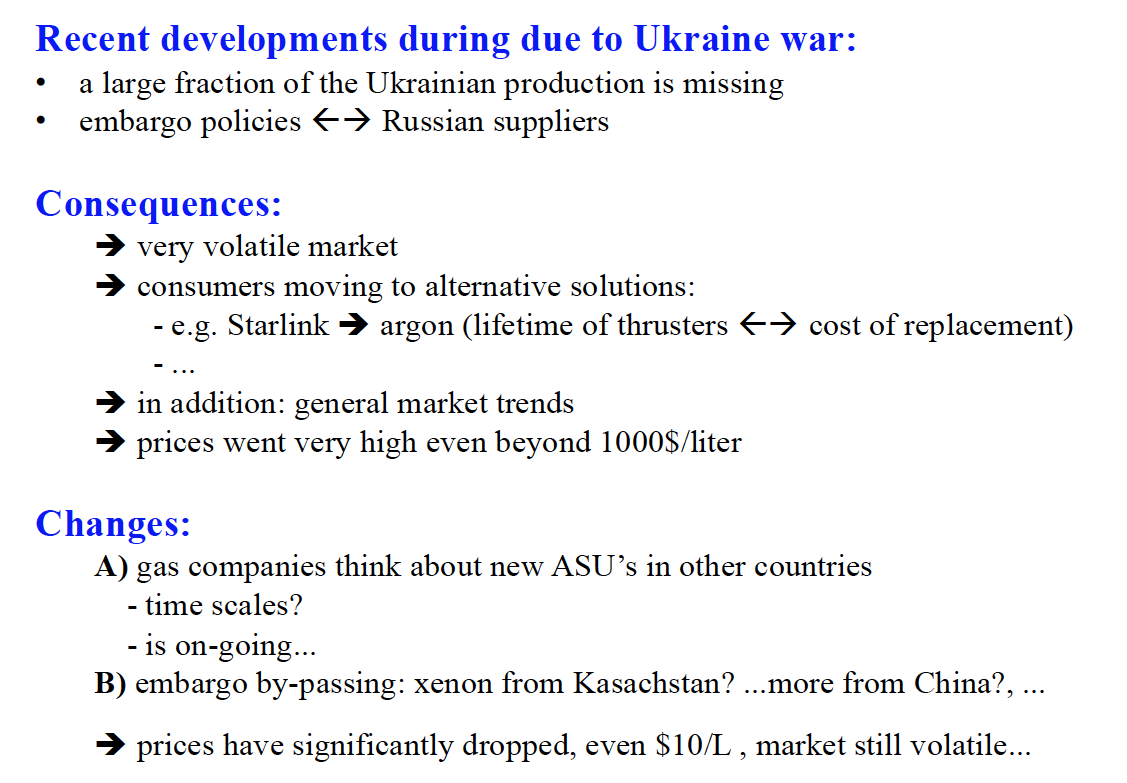
\includegraphics[scale=0.25]{volatile.png}
\end{frame}


\begin{frame}{Supply versus Demand}
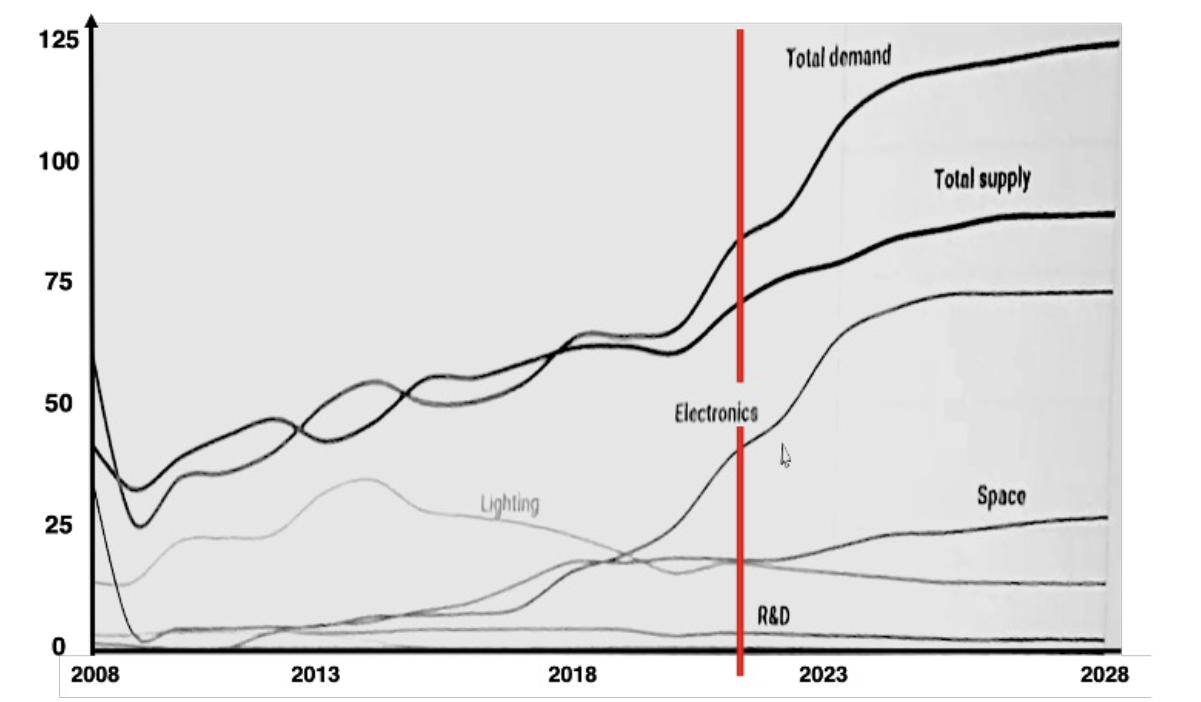
\includegraphics[scale=0.30]{xedemand.png}
\end{frame}


\begin{frame}{Xenon Price}
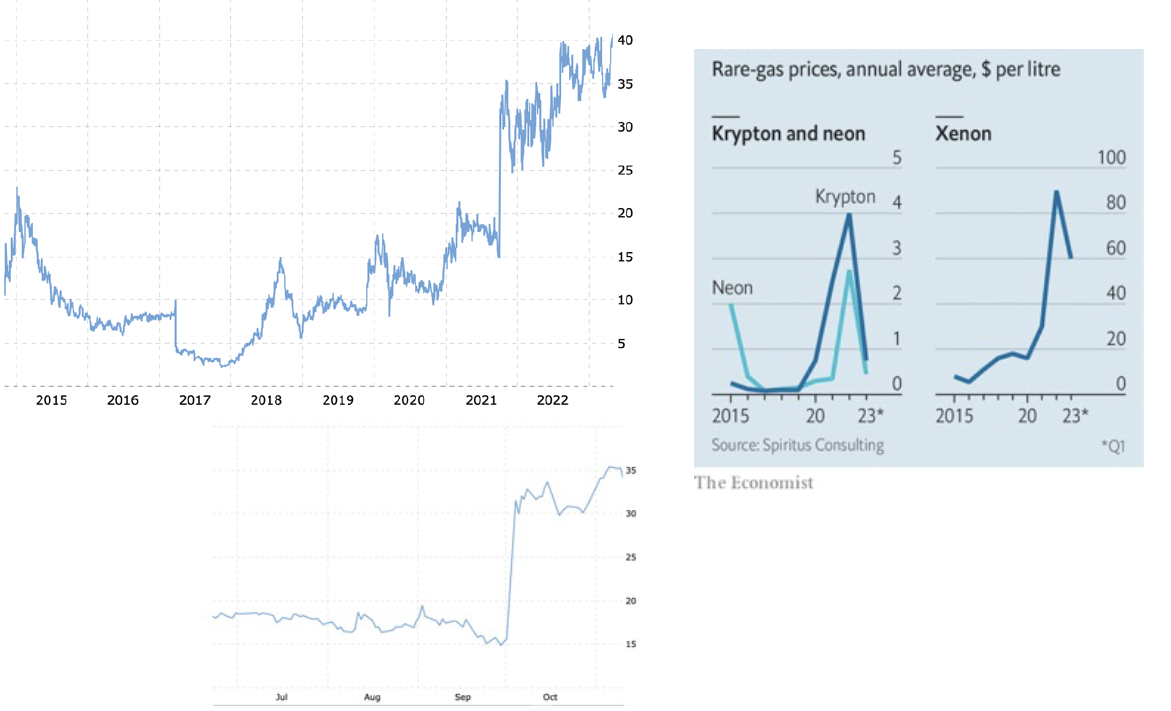
\includegraphics[scale=0.30]{xeprice.png}
\end{frame}


\begin{frame}{Ionisation and scintillation in Xe}
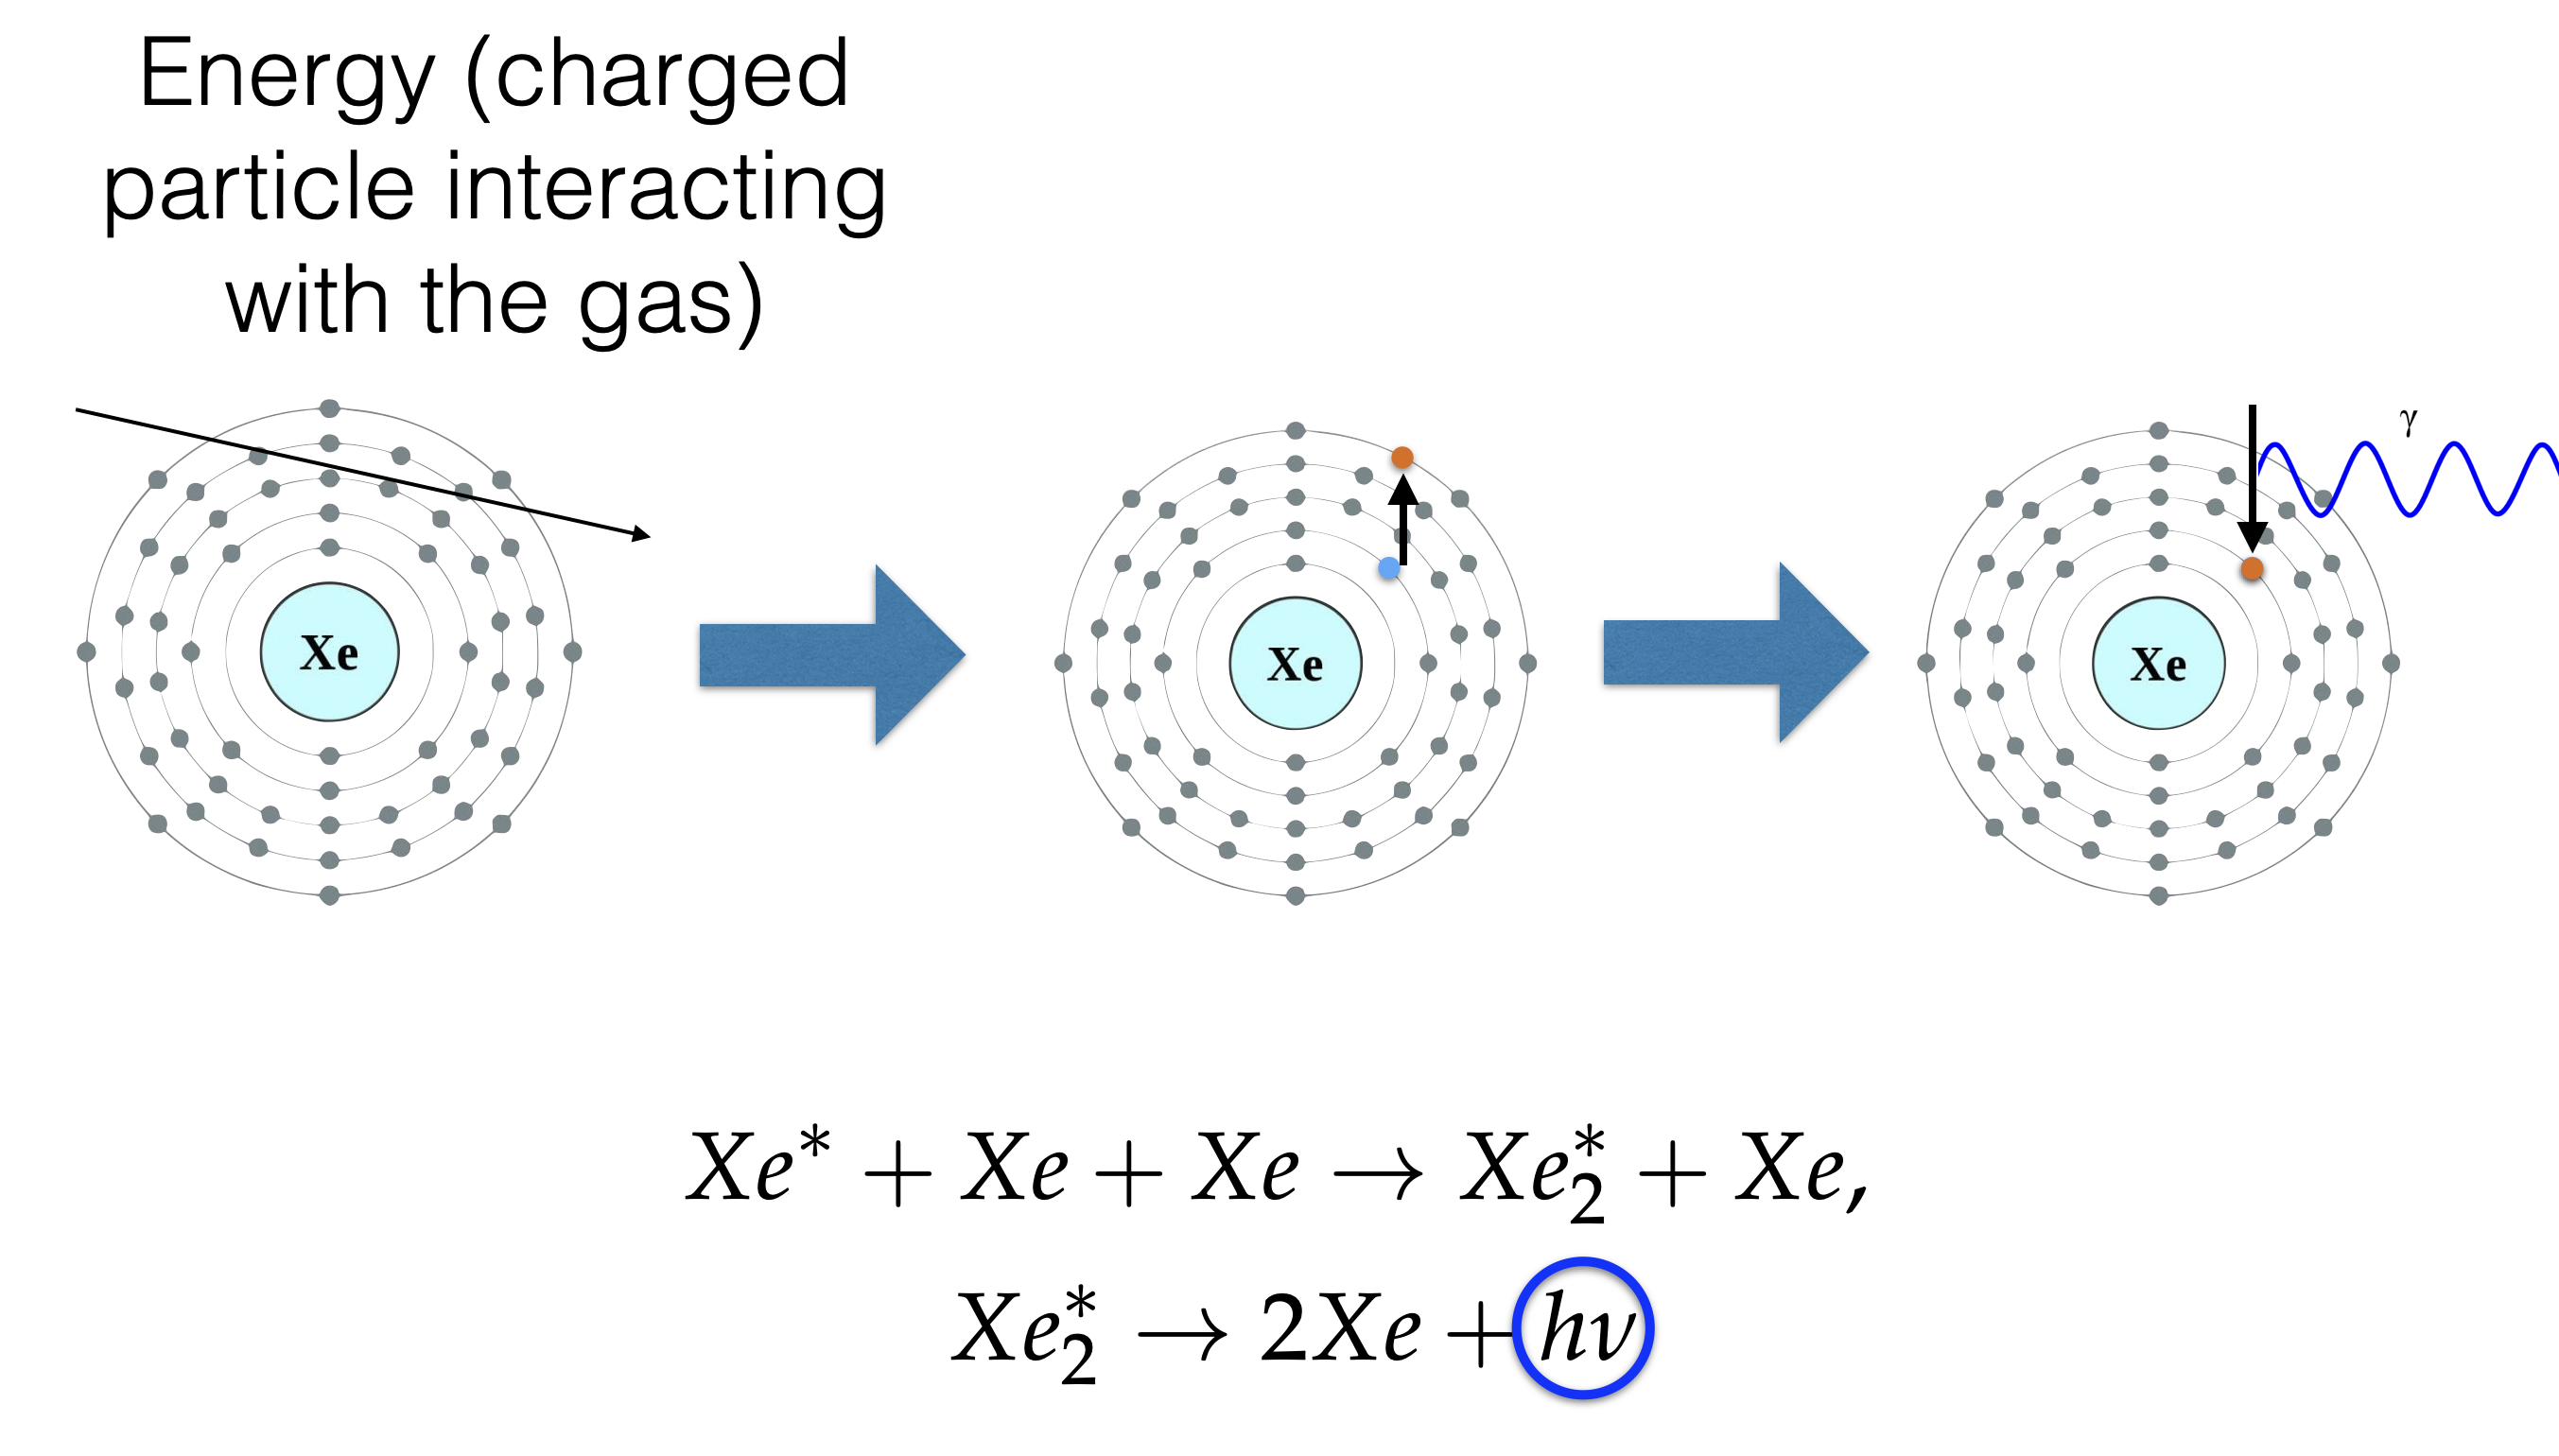
\includegraphics[scale=0.25]{xeio.png}
\end{frame}

\begin{frame}{Ionisation and scintillation in Xe}
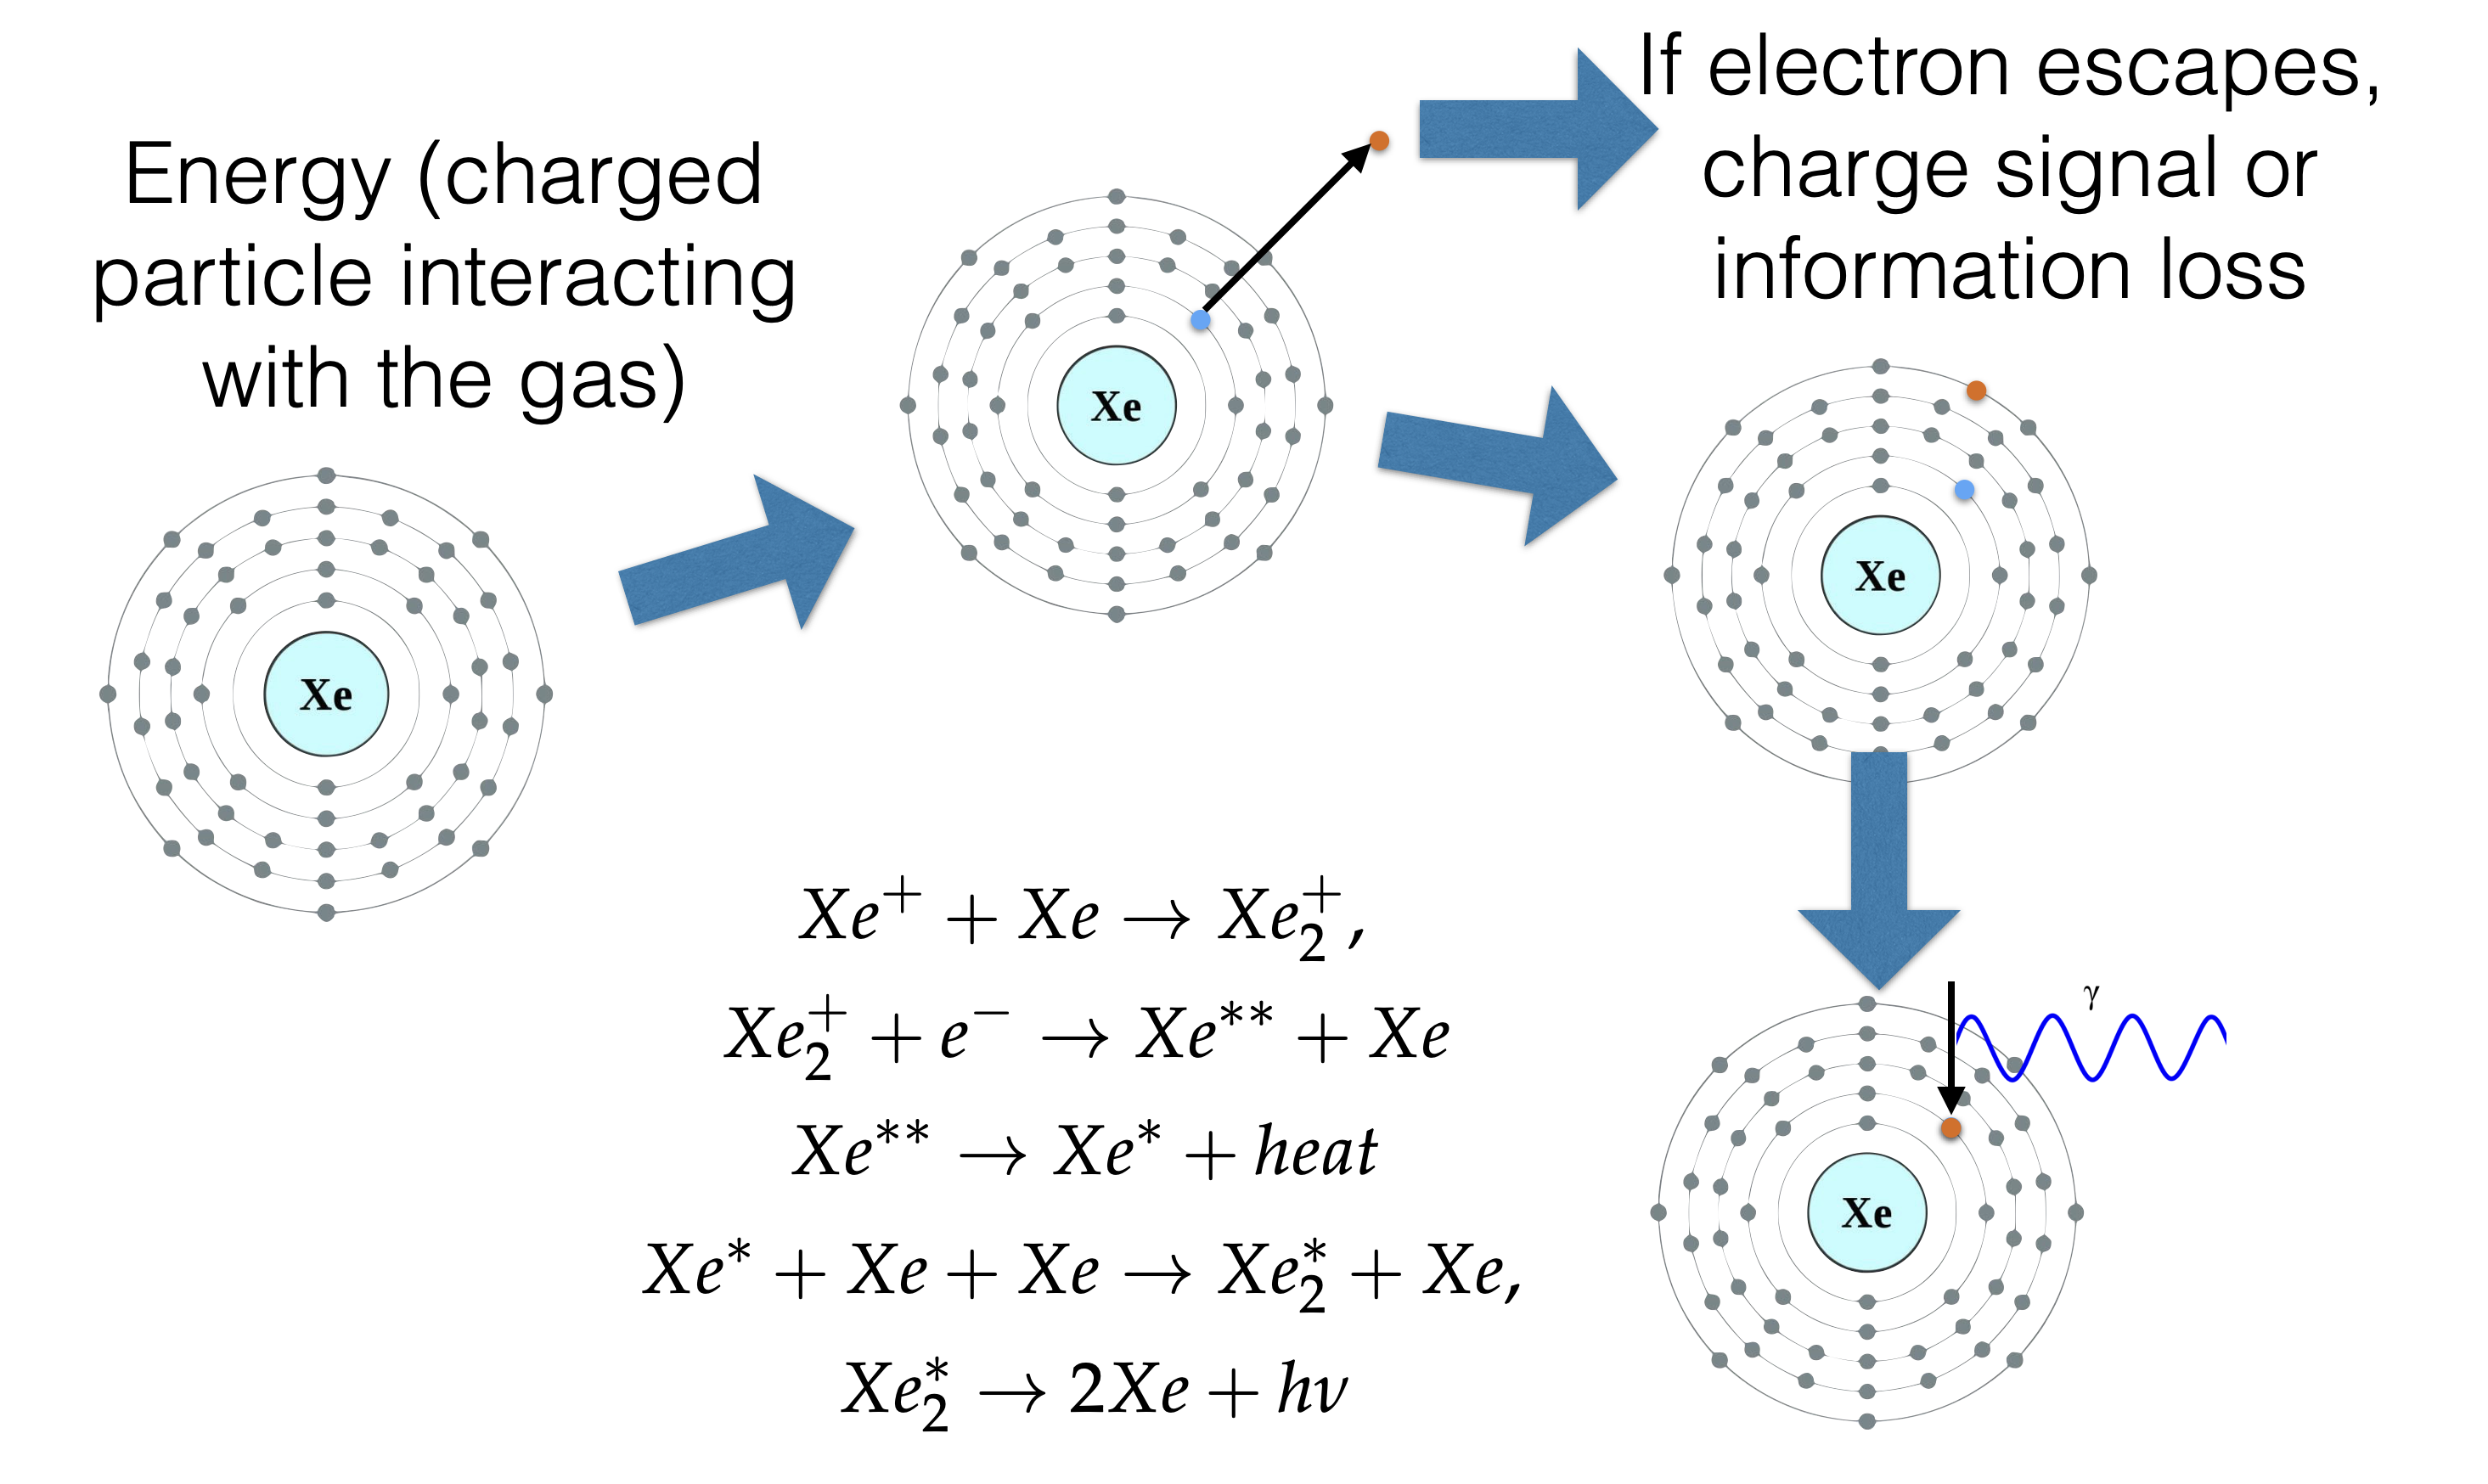
\includegraphics[scale=0.25]{xeio2.png}
\end{frame}

\begin{frame}{Ionisation and scintillation in Xe}
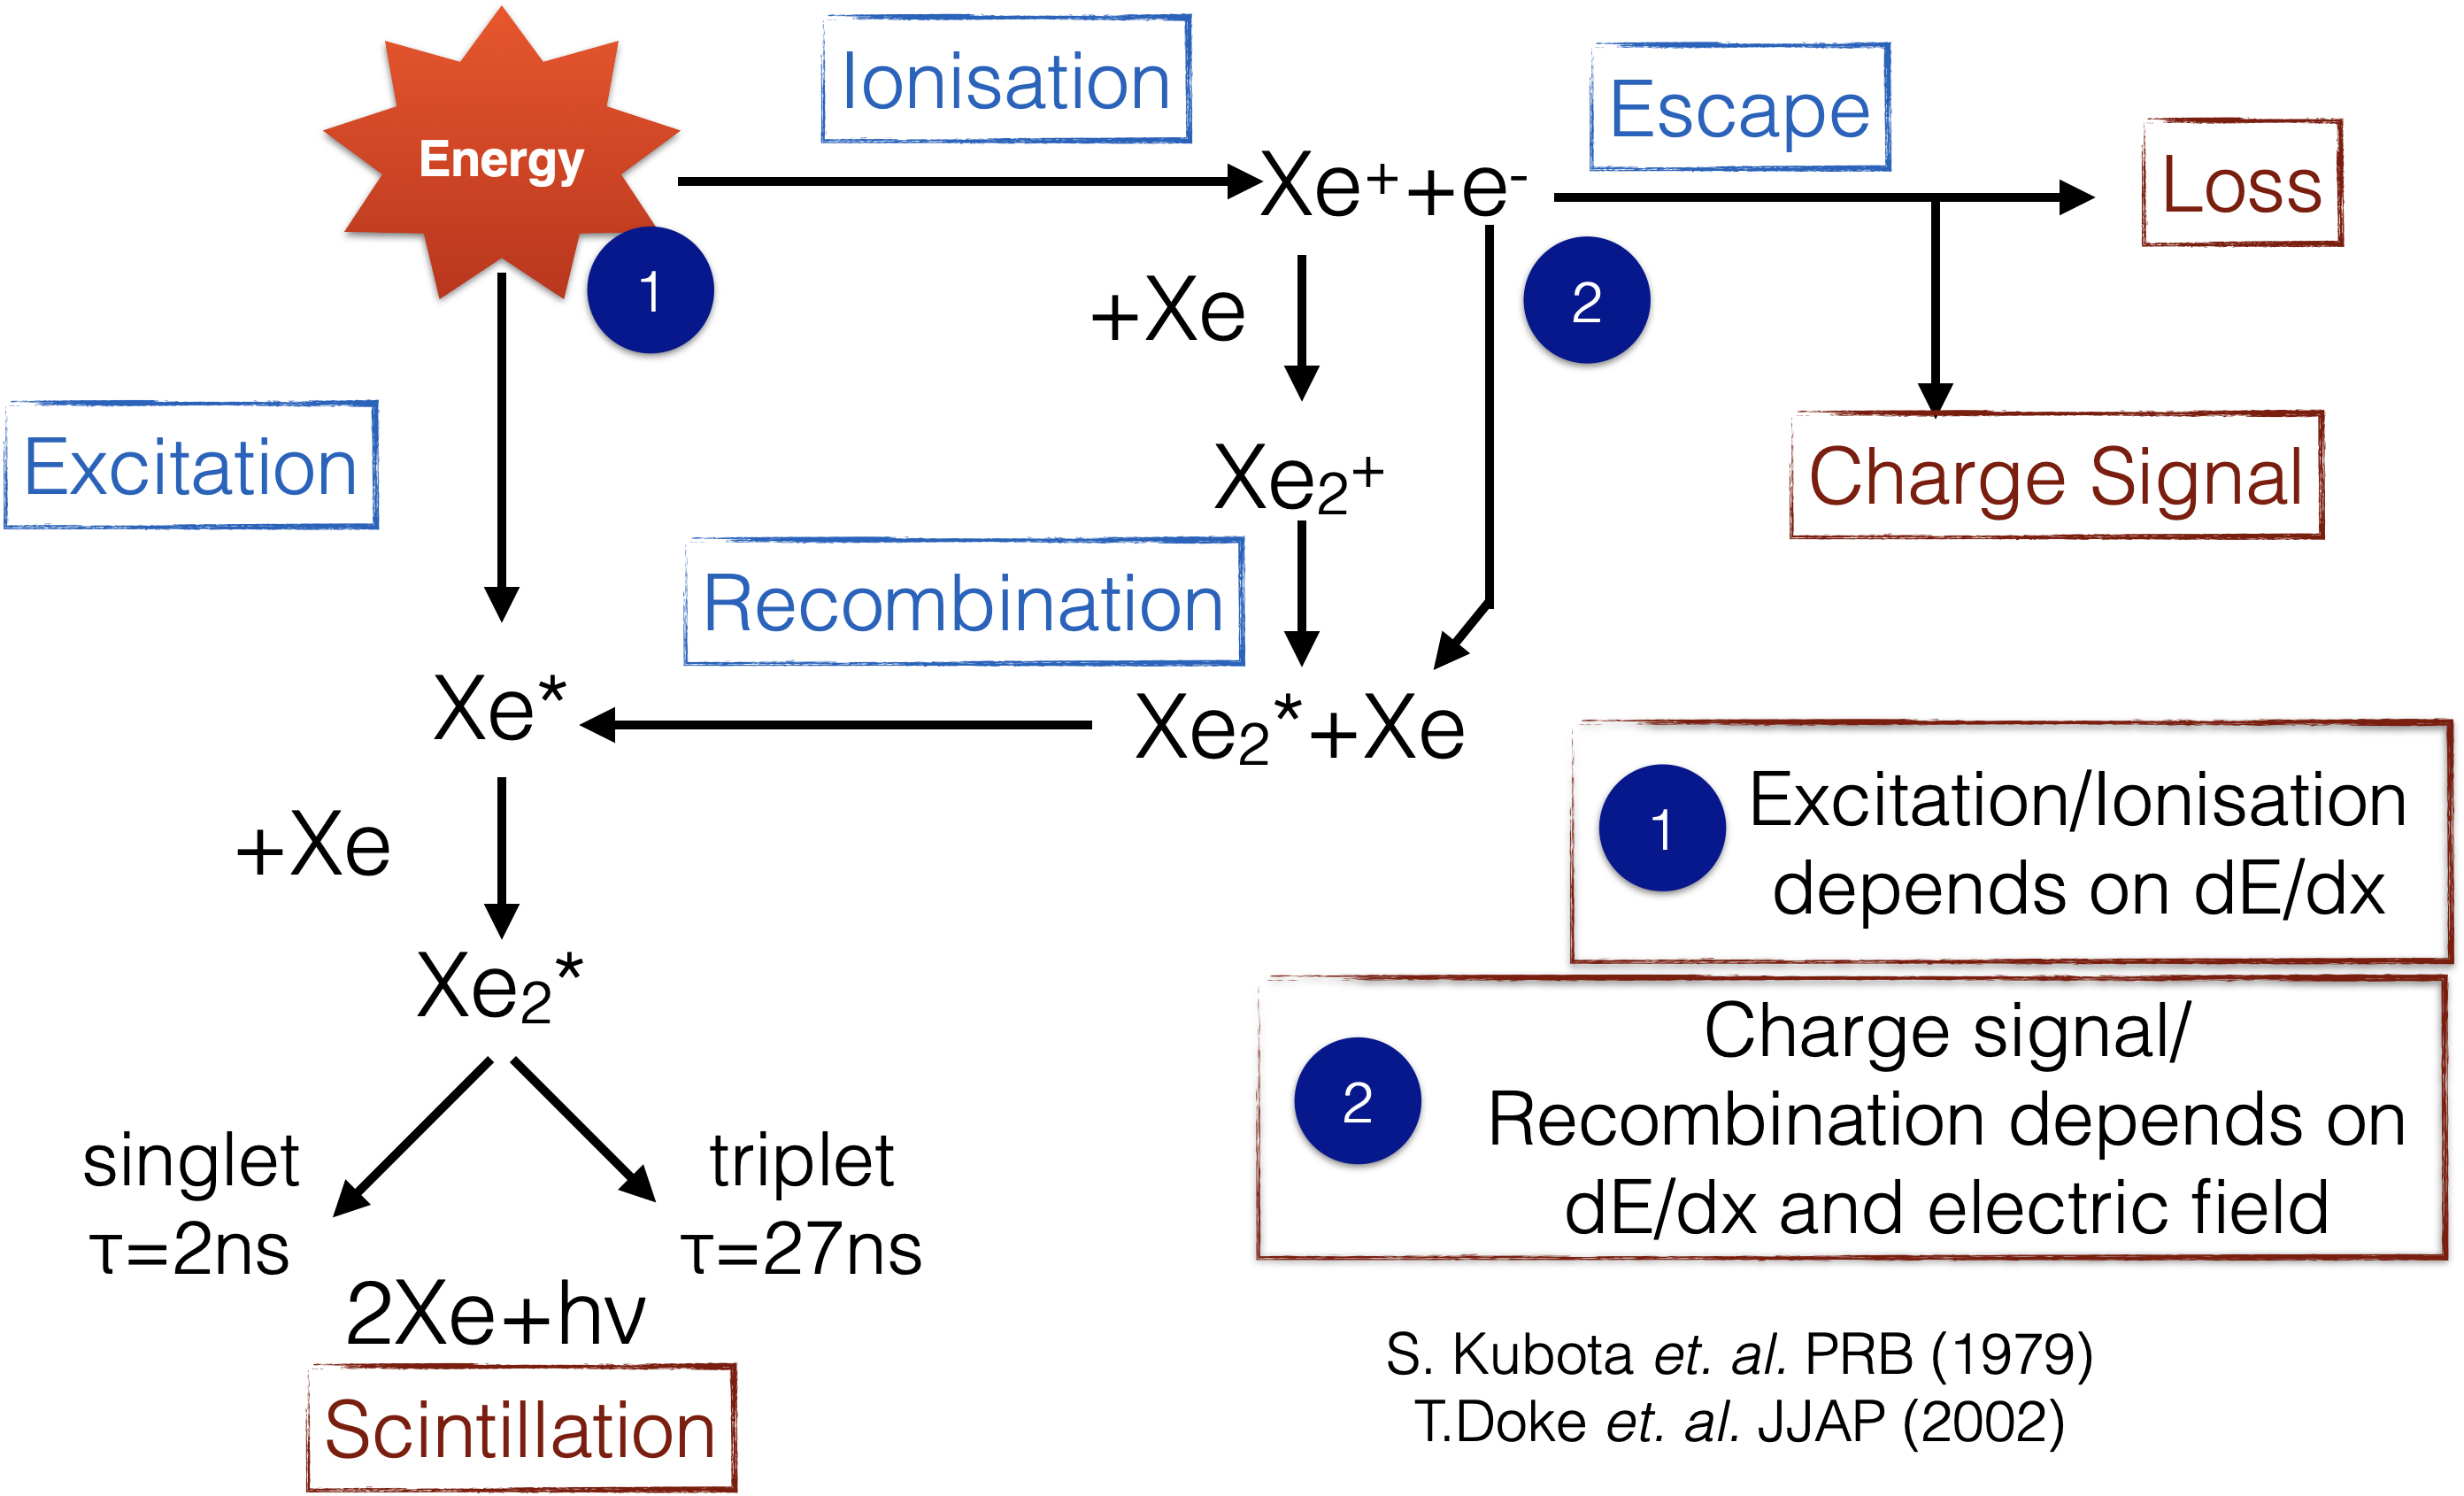
\includegraphics[scale=0.25]{xeio3.png}
\end{frame}

\begin{frame}{Anticorrelation between ionisation and scintillation in Xe}
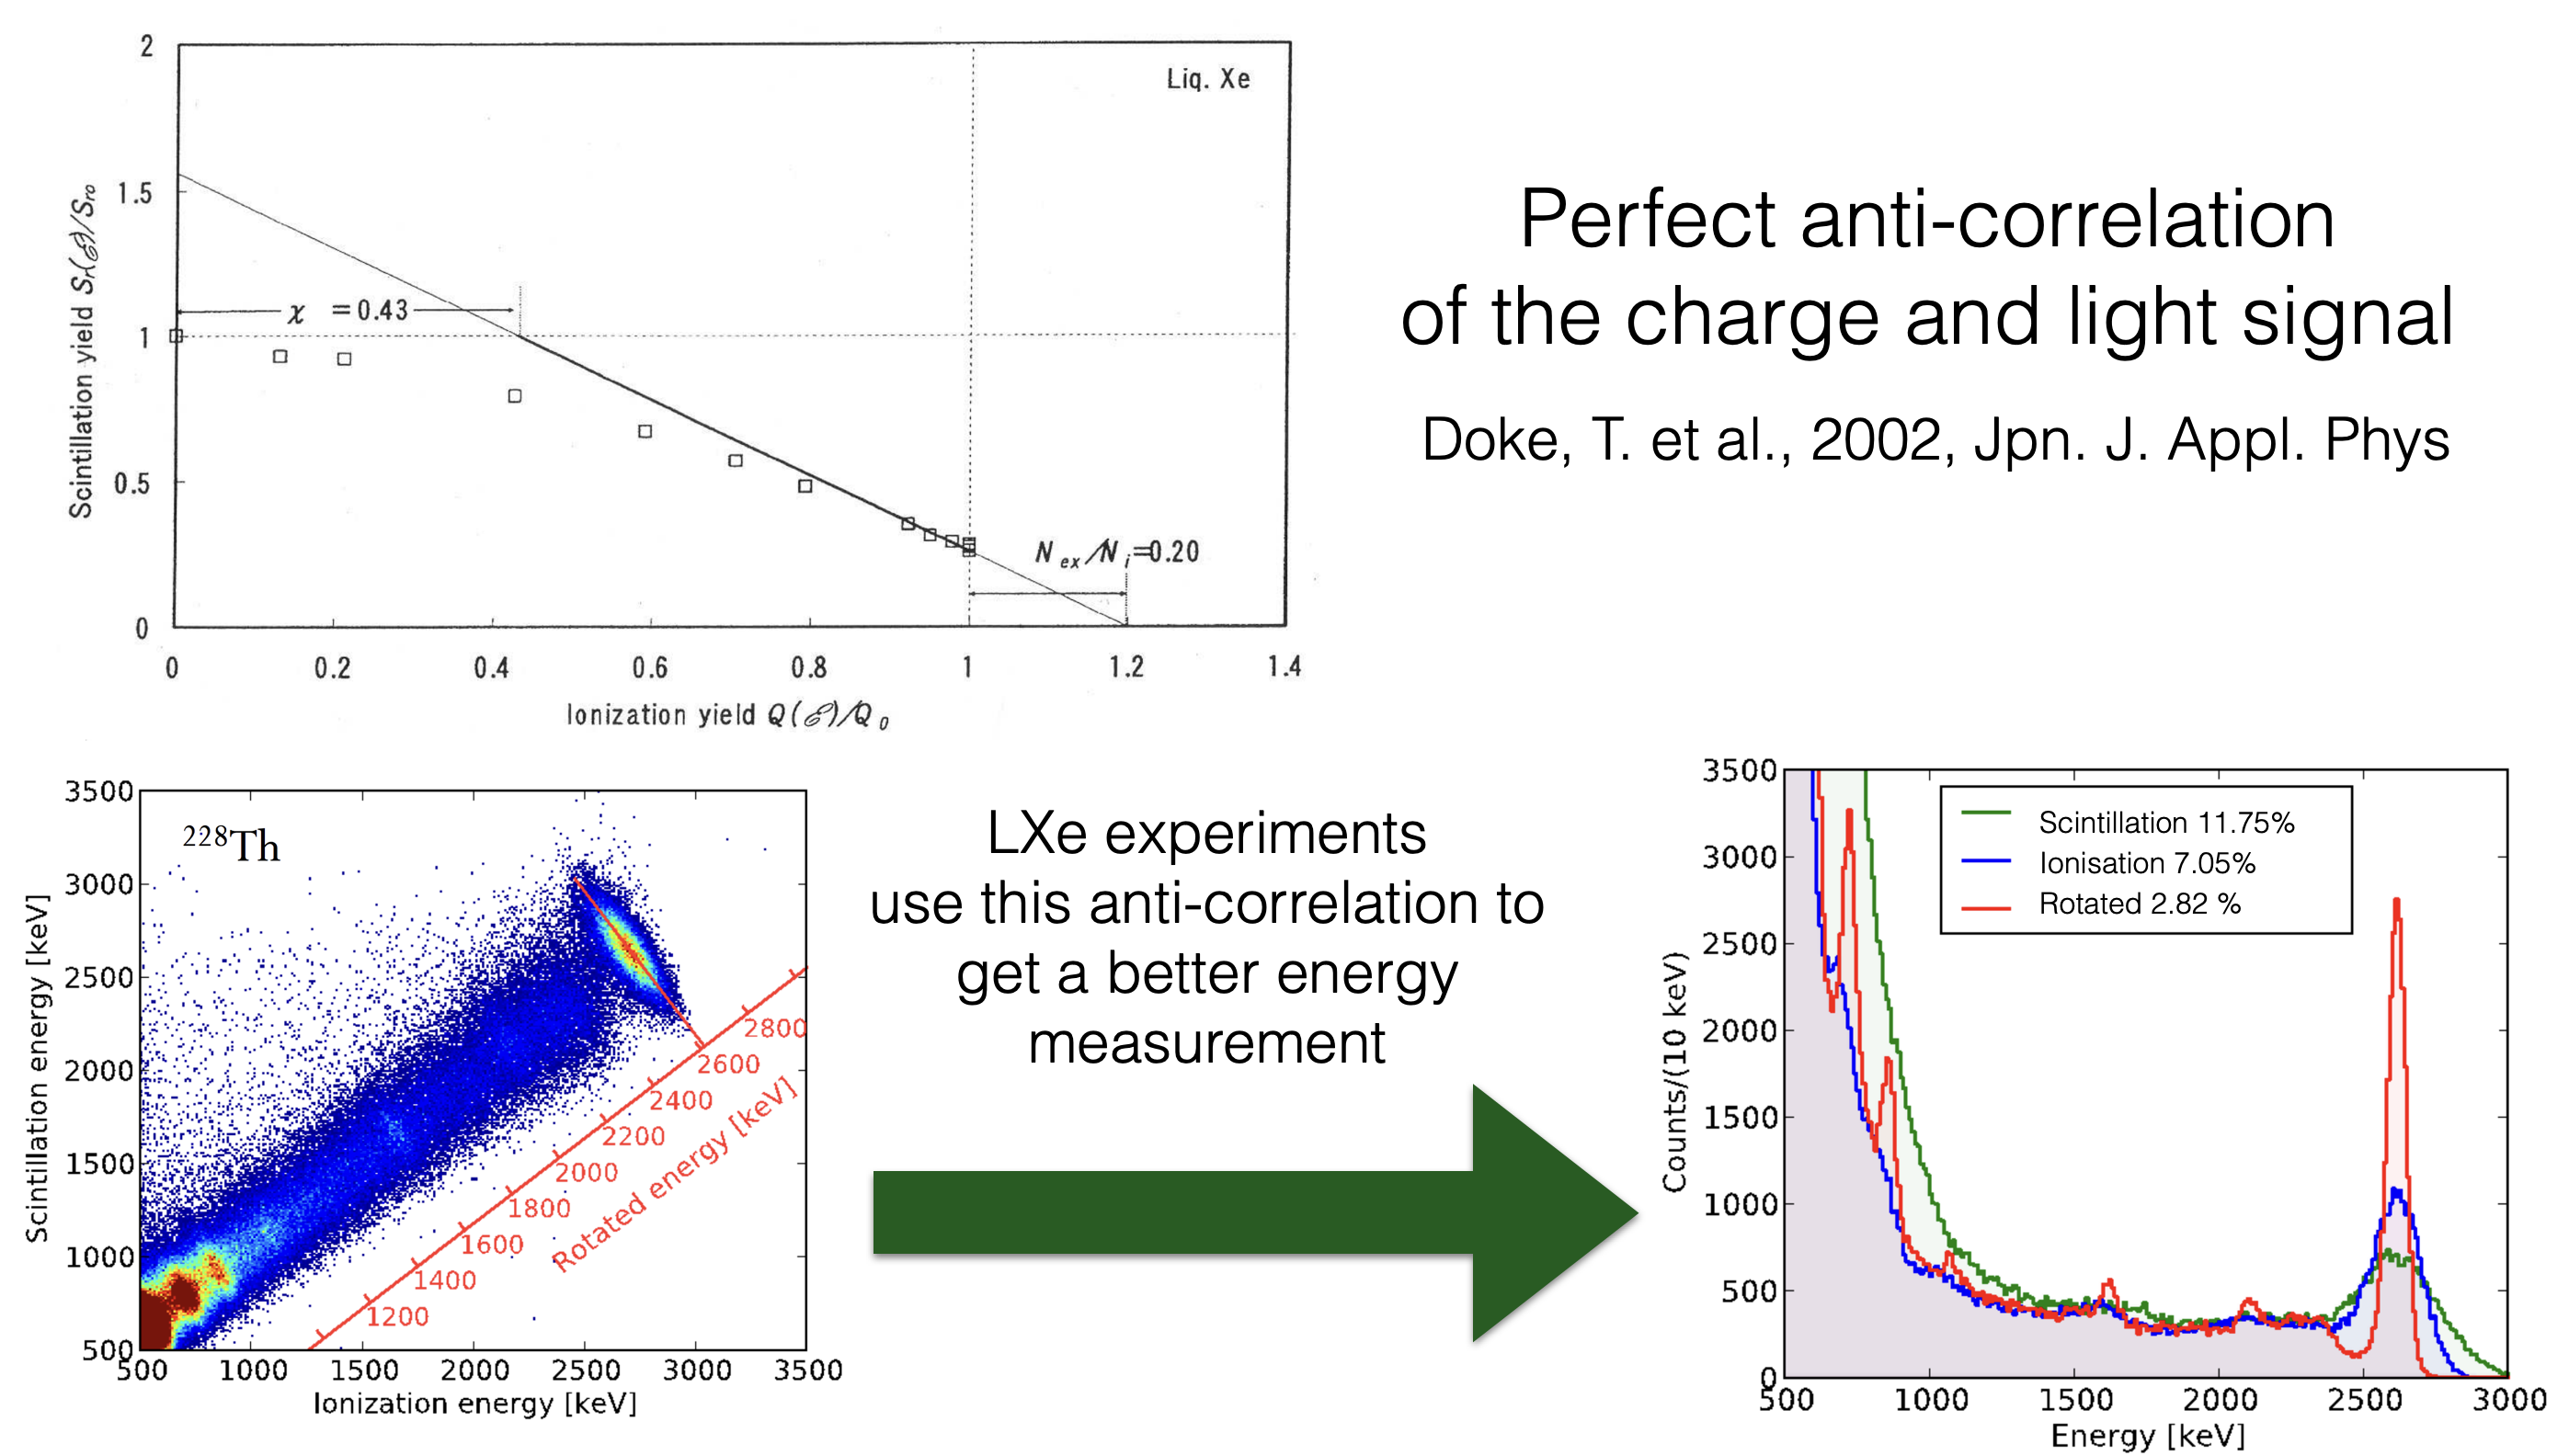
\includegraphics[scale=0.25]{anticorr.png}
\end{frame}

\begin{frame}{\XE\ is a good isotope for \bbonu\ searches}
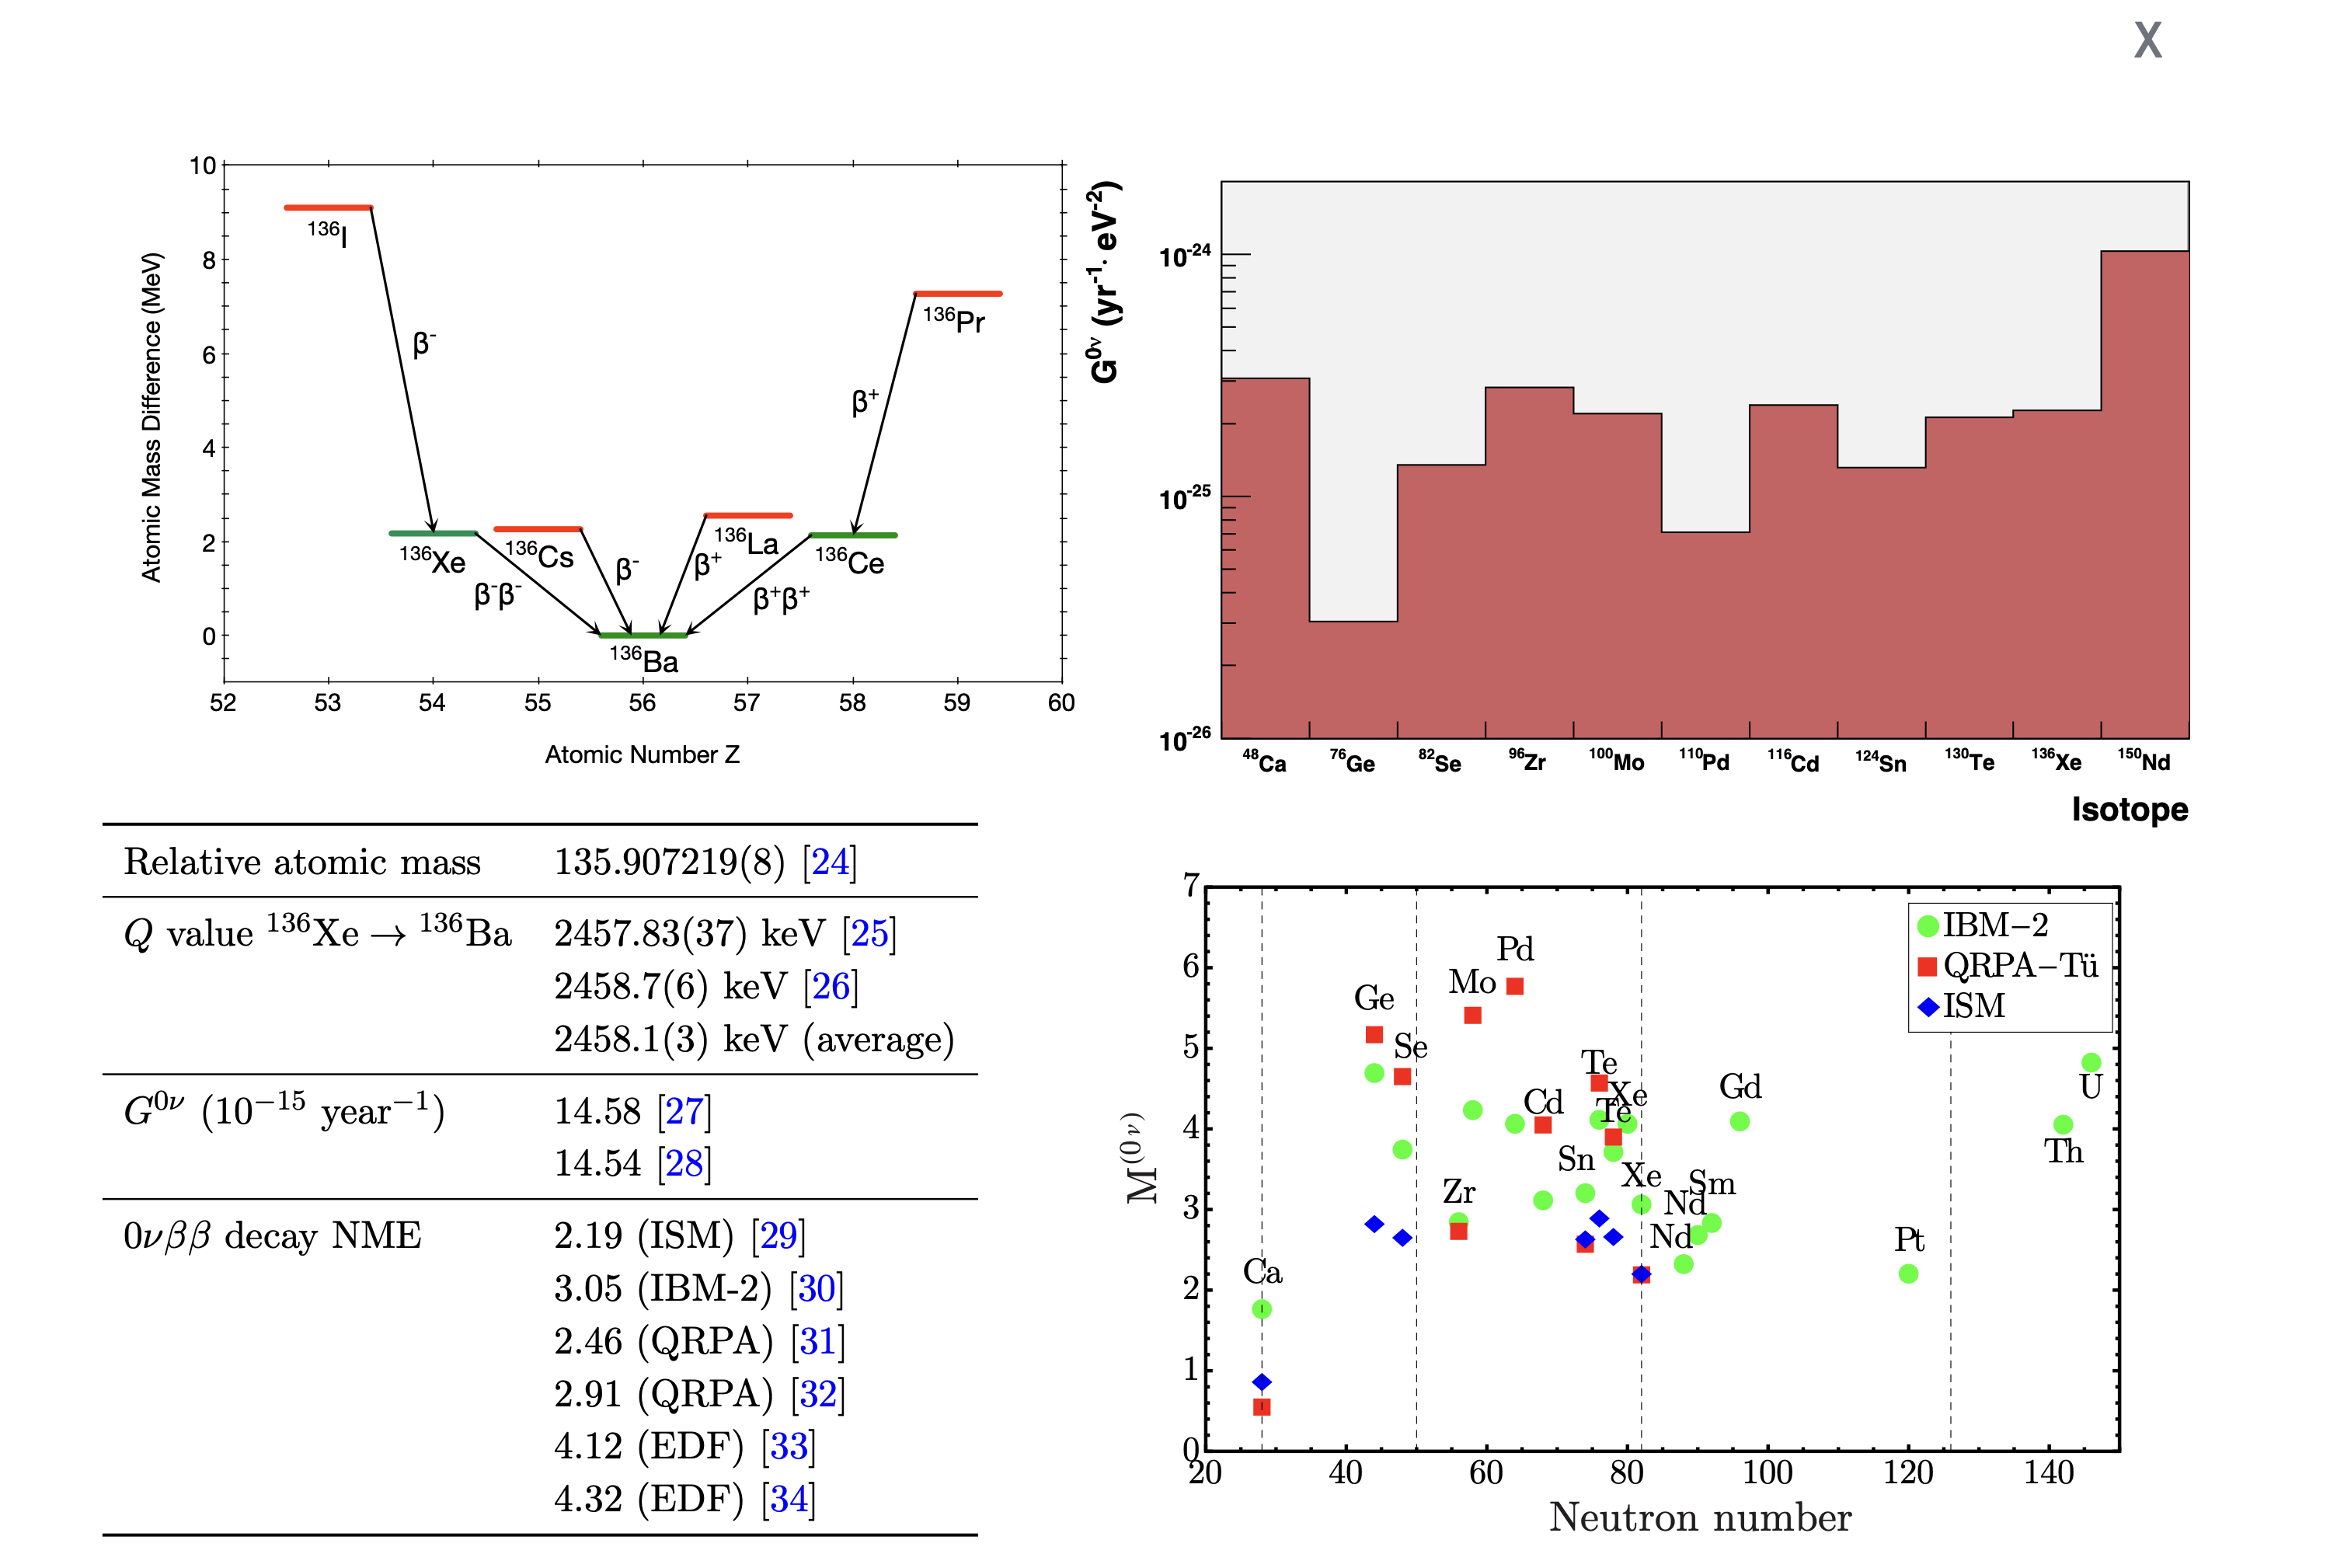
\includegraphics[scale=0.22]{xebb0nu.png}
\end{frame}

\begin{frame}{\XE\ is a good isotope for \bbonu\ searches}
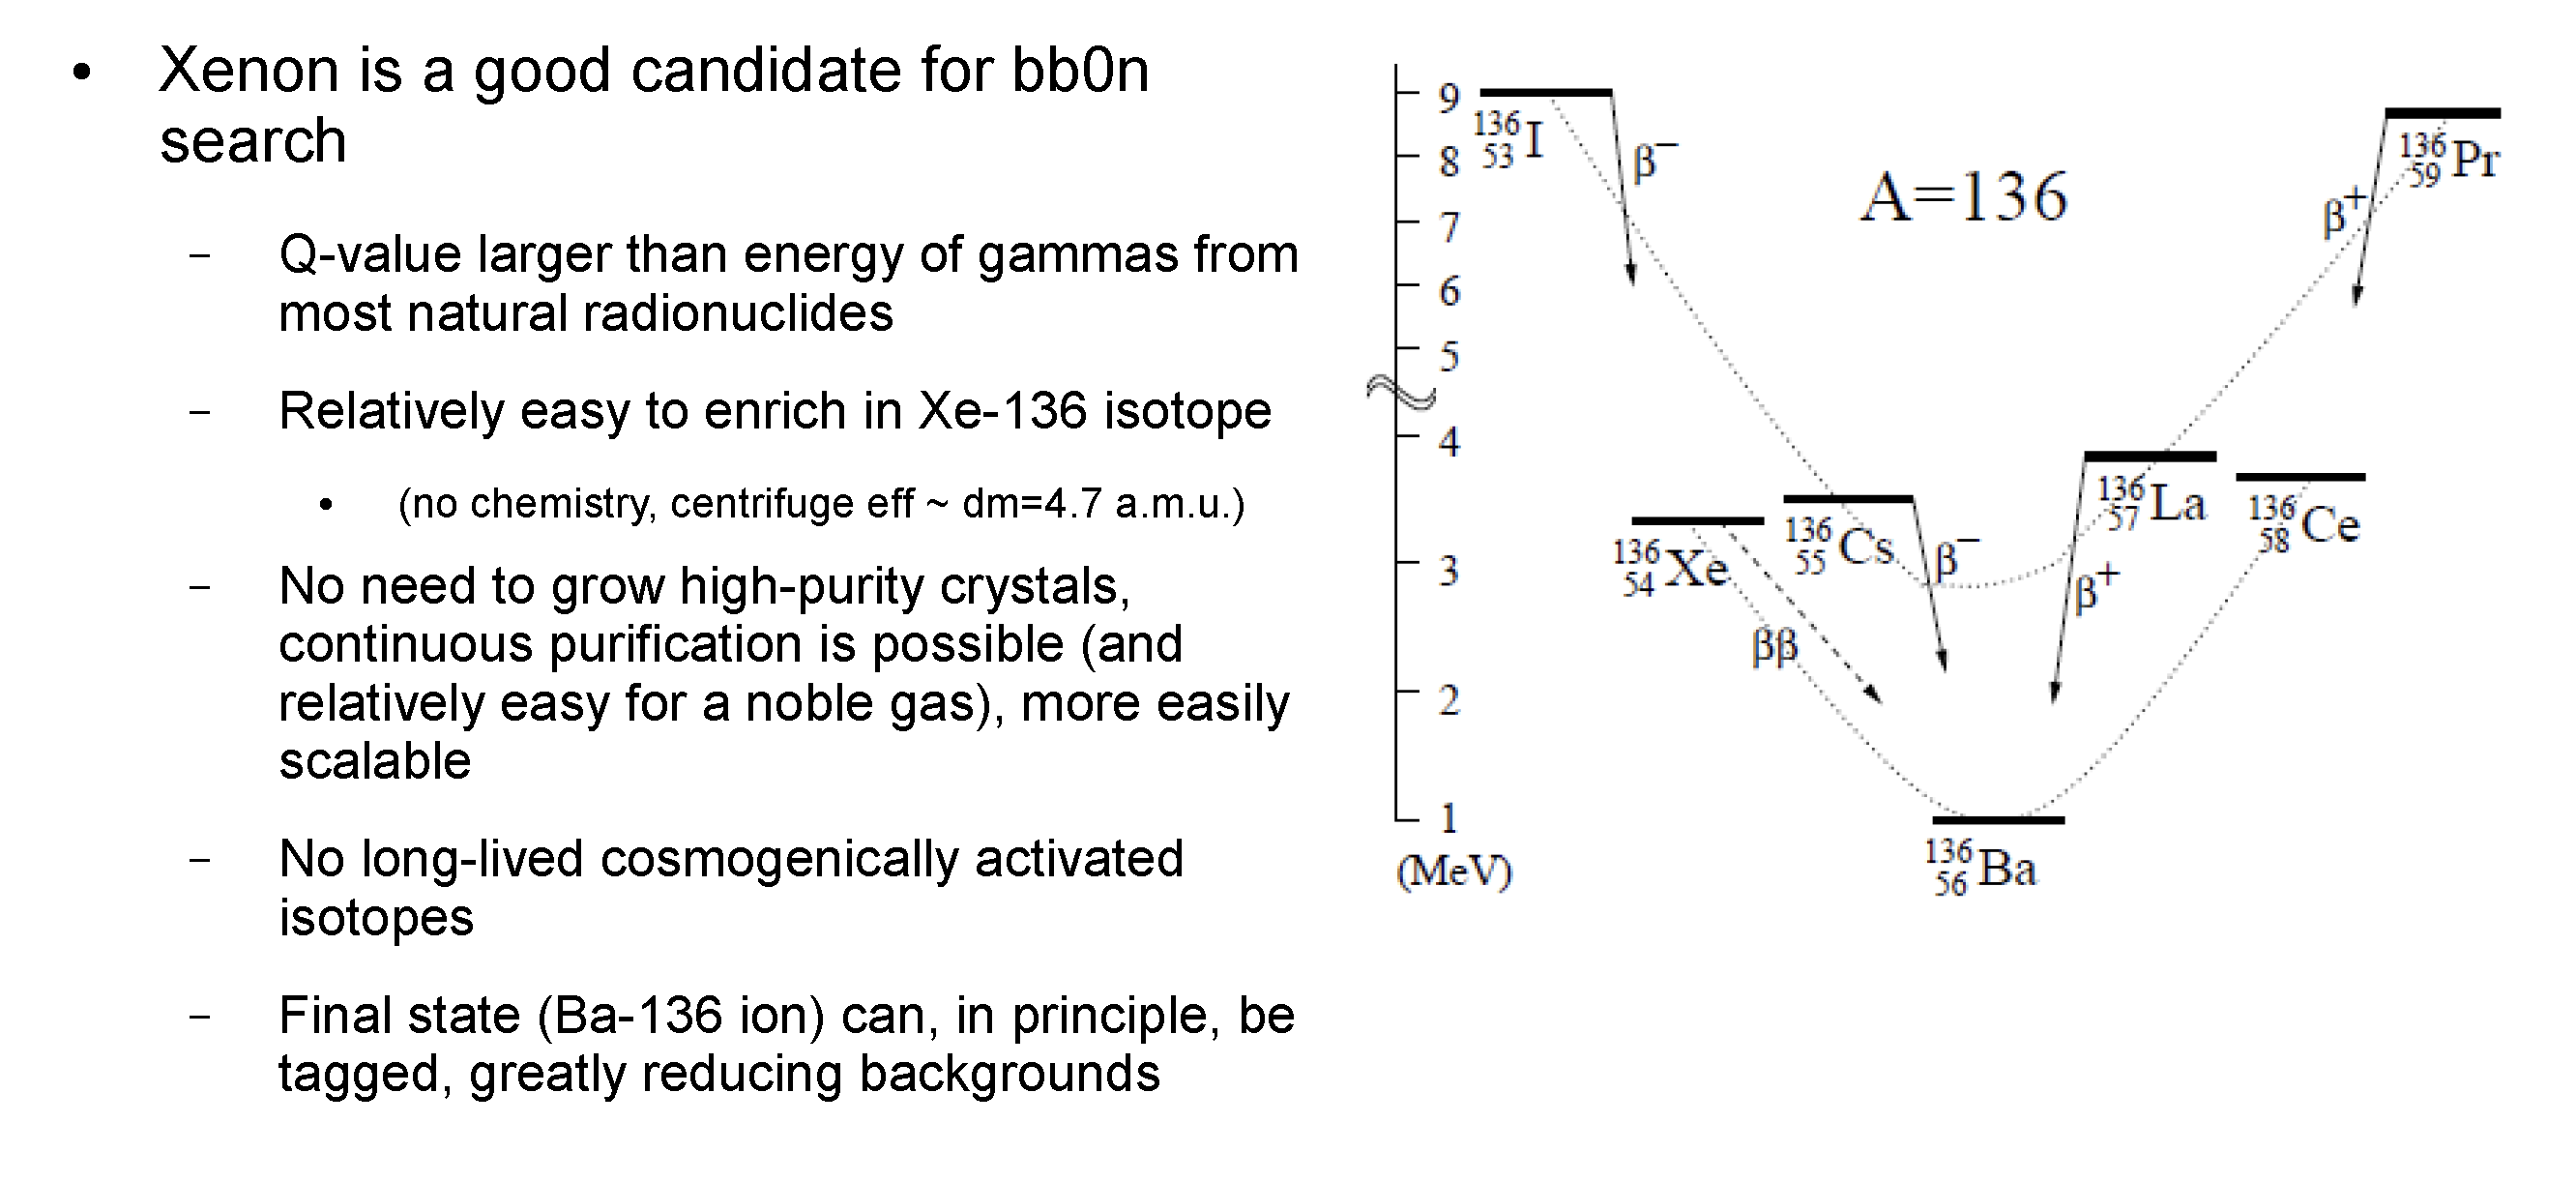
\includegraphics[scale=0.42]{xenonbbonu2.png}
\end{frame}

\begin{frame}{Exercise 1}
$\bullet~$ How much money would you need to buy the raw material for your ultimate \bbonu\  experiment in 2017?  And in 2023? Assume you will need O(100) tons of Xe.
\end{frame}



%%%%%%%%
%\begin{frame}{Ionisation and scintillation in Xe}
%$\bullet$~When a charged particle propagates through a noble gas the Coulomb interaction with the atoms result in ionisation of the medium, releasing on average \nne\ electron-ion pairs:
%
%\[
%\nne = \frac{E}{W_I}
%\]
%where $E$ is the energy deposited by in the medium and $W_I$ is the average energy required to produce one electron-ion pair. In xenon gas $W_I=21.9$~eV (\url{https://arxiv.org/abs/1903.02435})
%
%
%$\bullet$~ The propagation of a charged particle in a noble gas also results in the emission of VUV scintillation
%light (with an average wavelength of 172 nm in xenon). Defining $W_s$ as the average energy needed in the
%creation of one primary scintillation photon, the average number of scintillation photons produced when a
%particle releases its energy E in the gas is:
%
%\[
%\nng = \frac{E}{W_s}
%\]
%In xenon gas $W_s =76 \pm 6$~eV (NEXT collaboration). 
%\end{frame}
%
%%%%
%
%\begin{frame}{Gas Proportional Scintillation Chamber (GPSC)}
%\begin{columns}
%\column{0.40\textwidth}
%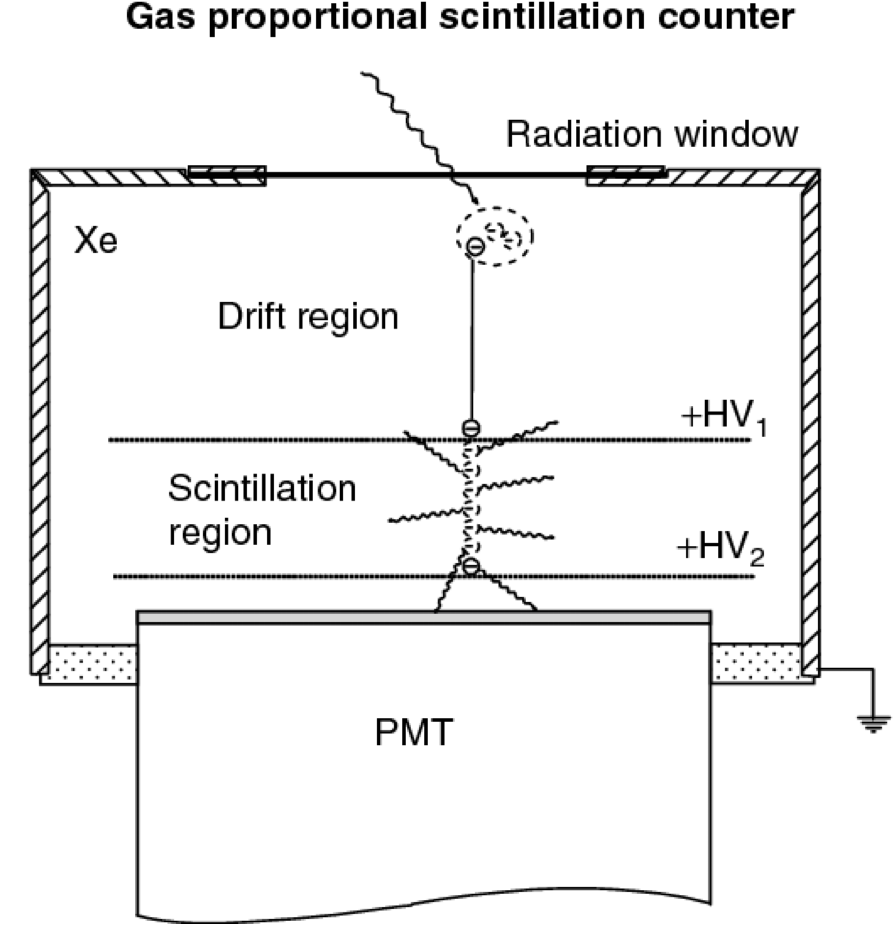
\includegraphics[scale=0.30]{gpsc.png}
%
% \column{0.60\textwidth}
%
%$\bullet~$ The principle of the GPSC (Conde and Policarpo, 1967) is as follows. An X-ray enters through the chamber window and is absorbed in a region of weak electric field known as the drift region. 
%
%$\bullet~$ The ionisation electrons drift under such field to a region
%of moderately high electric field (around 3 kV cm$^{-1}\cdot$ bar$^{-1}$ the so-called scintillation or EL region. 
%
%$\bullet~$ There, each electron is accelerated so that it excites, but does not ionise, the gas atoms/molecules. The excited
%atoms decay, emitting UV light (the so-called secondary scintillation), which is detected by photosensors.
%\end{columns}
%\end{frame}
%
%%%%%%
%\begin{frame}{Electroluminescence yield}
%$\bullet$~Monte Carlo calculation (Oliveira et al):
%
%\[
%(\frac{Y}{p})= (130 \pm 1) (\frac{E}{p}) - (80 \pm 3) {\rm [photons electron^{-1} cm^{-1} bar^{-1}]}
%\]
%where the reduced electroluminescence yield is defined as the number of photons emitted per primary
%electron and per unit of drift length divided by the pressure of the gas, and$E/p$ is expressed in
%kV$\cdot$cm$^{-1}\cdot$bar$^{-1}$. The formula was found to be in good agreement with experimental data measured at 1 bar. 
%
%$\bullet$~ {\bf Exercise 10}. a) Plot the reduced yield as a function of $E/P$. 
%
%%$\bullet$~ {\bf Exercise 10}. a) Plot the reduced yield as a function of $E/P$. b) Select three different pressures, 5, 10 and 15 bar. Plot the yield as a function of the electric field. Suppose that you want to achieve an amplification of 10$^3$~photons per electron, with an amplification gap of 1 cm at 10 bar. Which EL electric field do you need? 
%\end{frame}
%
%%%%
%
%\begin{frame}{The Time projection chamber}
%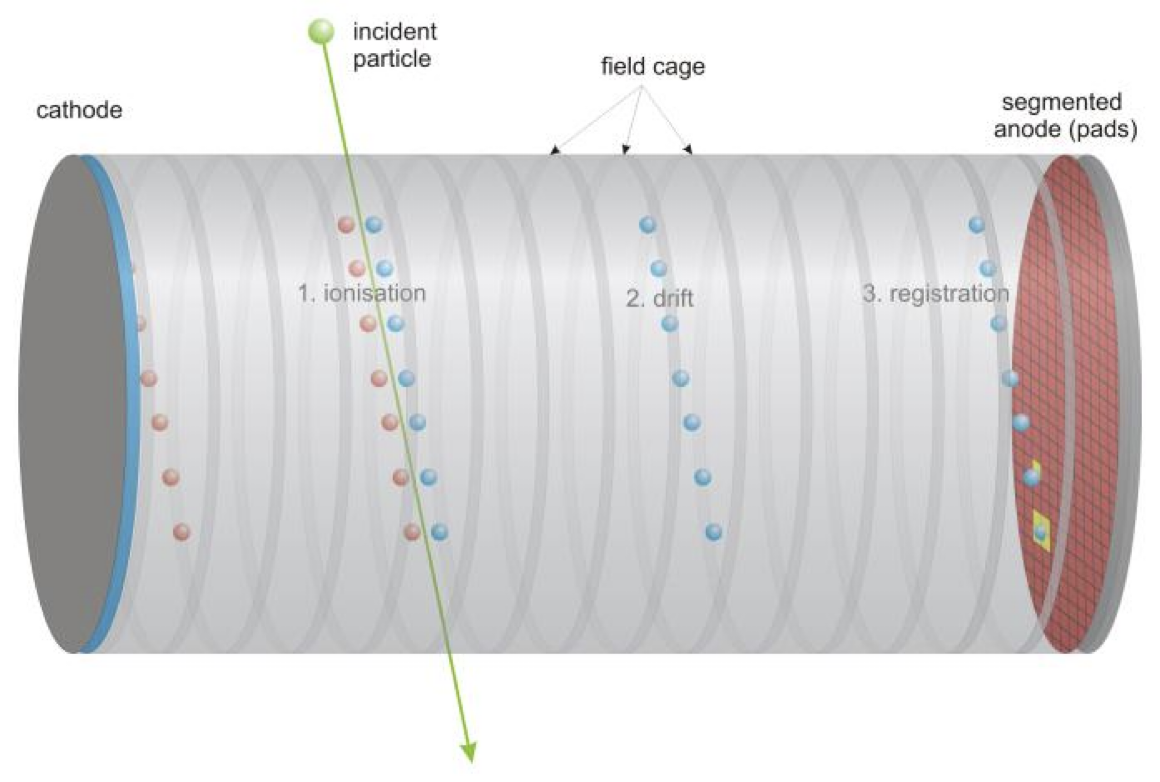
\includegraphics[scale=0.42]{tpc.png}
%
%$\bullet$~The Time Projection Chamber (TPC). Invented by Dave Nygren, is one of the most successful detectors in nuclear and particle physics. 
%It provides 3D image of tracks and if the track is contained also energy by calorimetric measurement. 
%\end{frame}
%%%%%
%
%\begin{frame}{The NEXT concept: A HPXe EL TPC}
%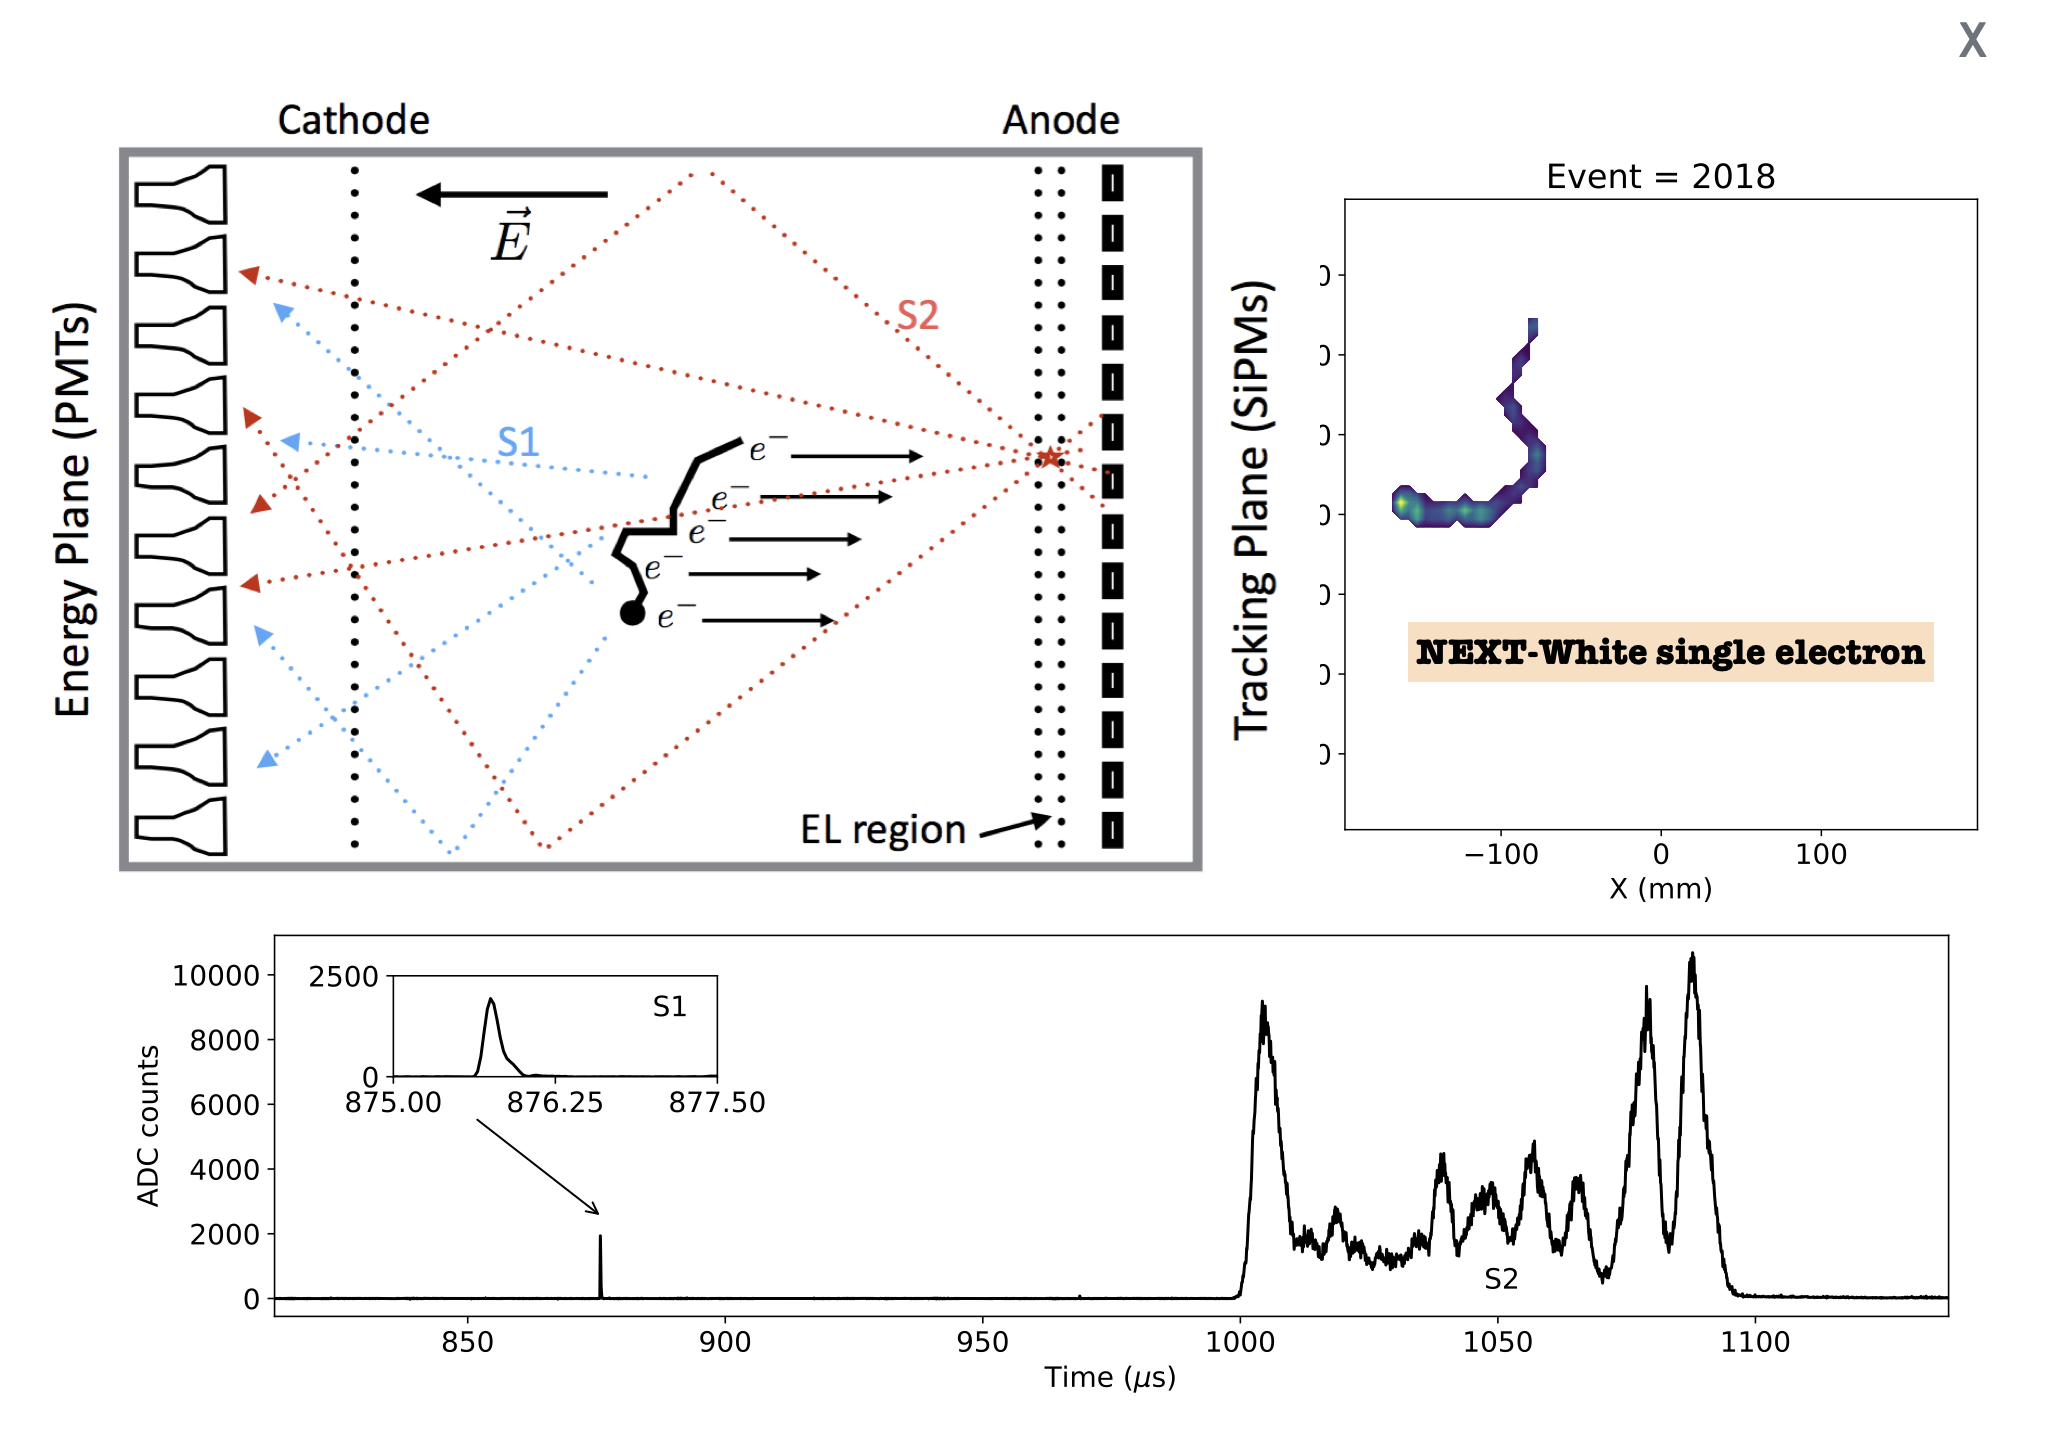
\includegraphics[scale=0.30]{nextpo.png}
% 
%\end{frame}
%
%%%%%%%
%\begin{frame}{The NEXT concept: A HPXe EL TPC}
%
%\begin{columns}
%\column{0.50\textwidth}
%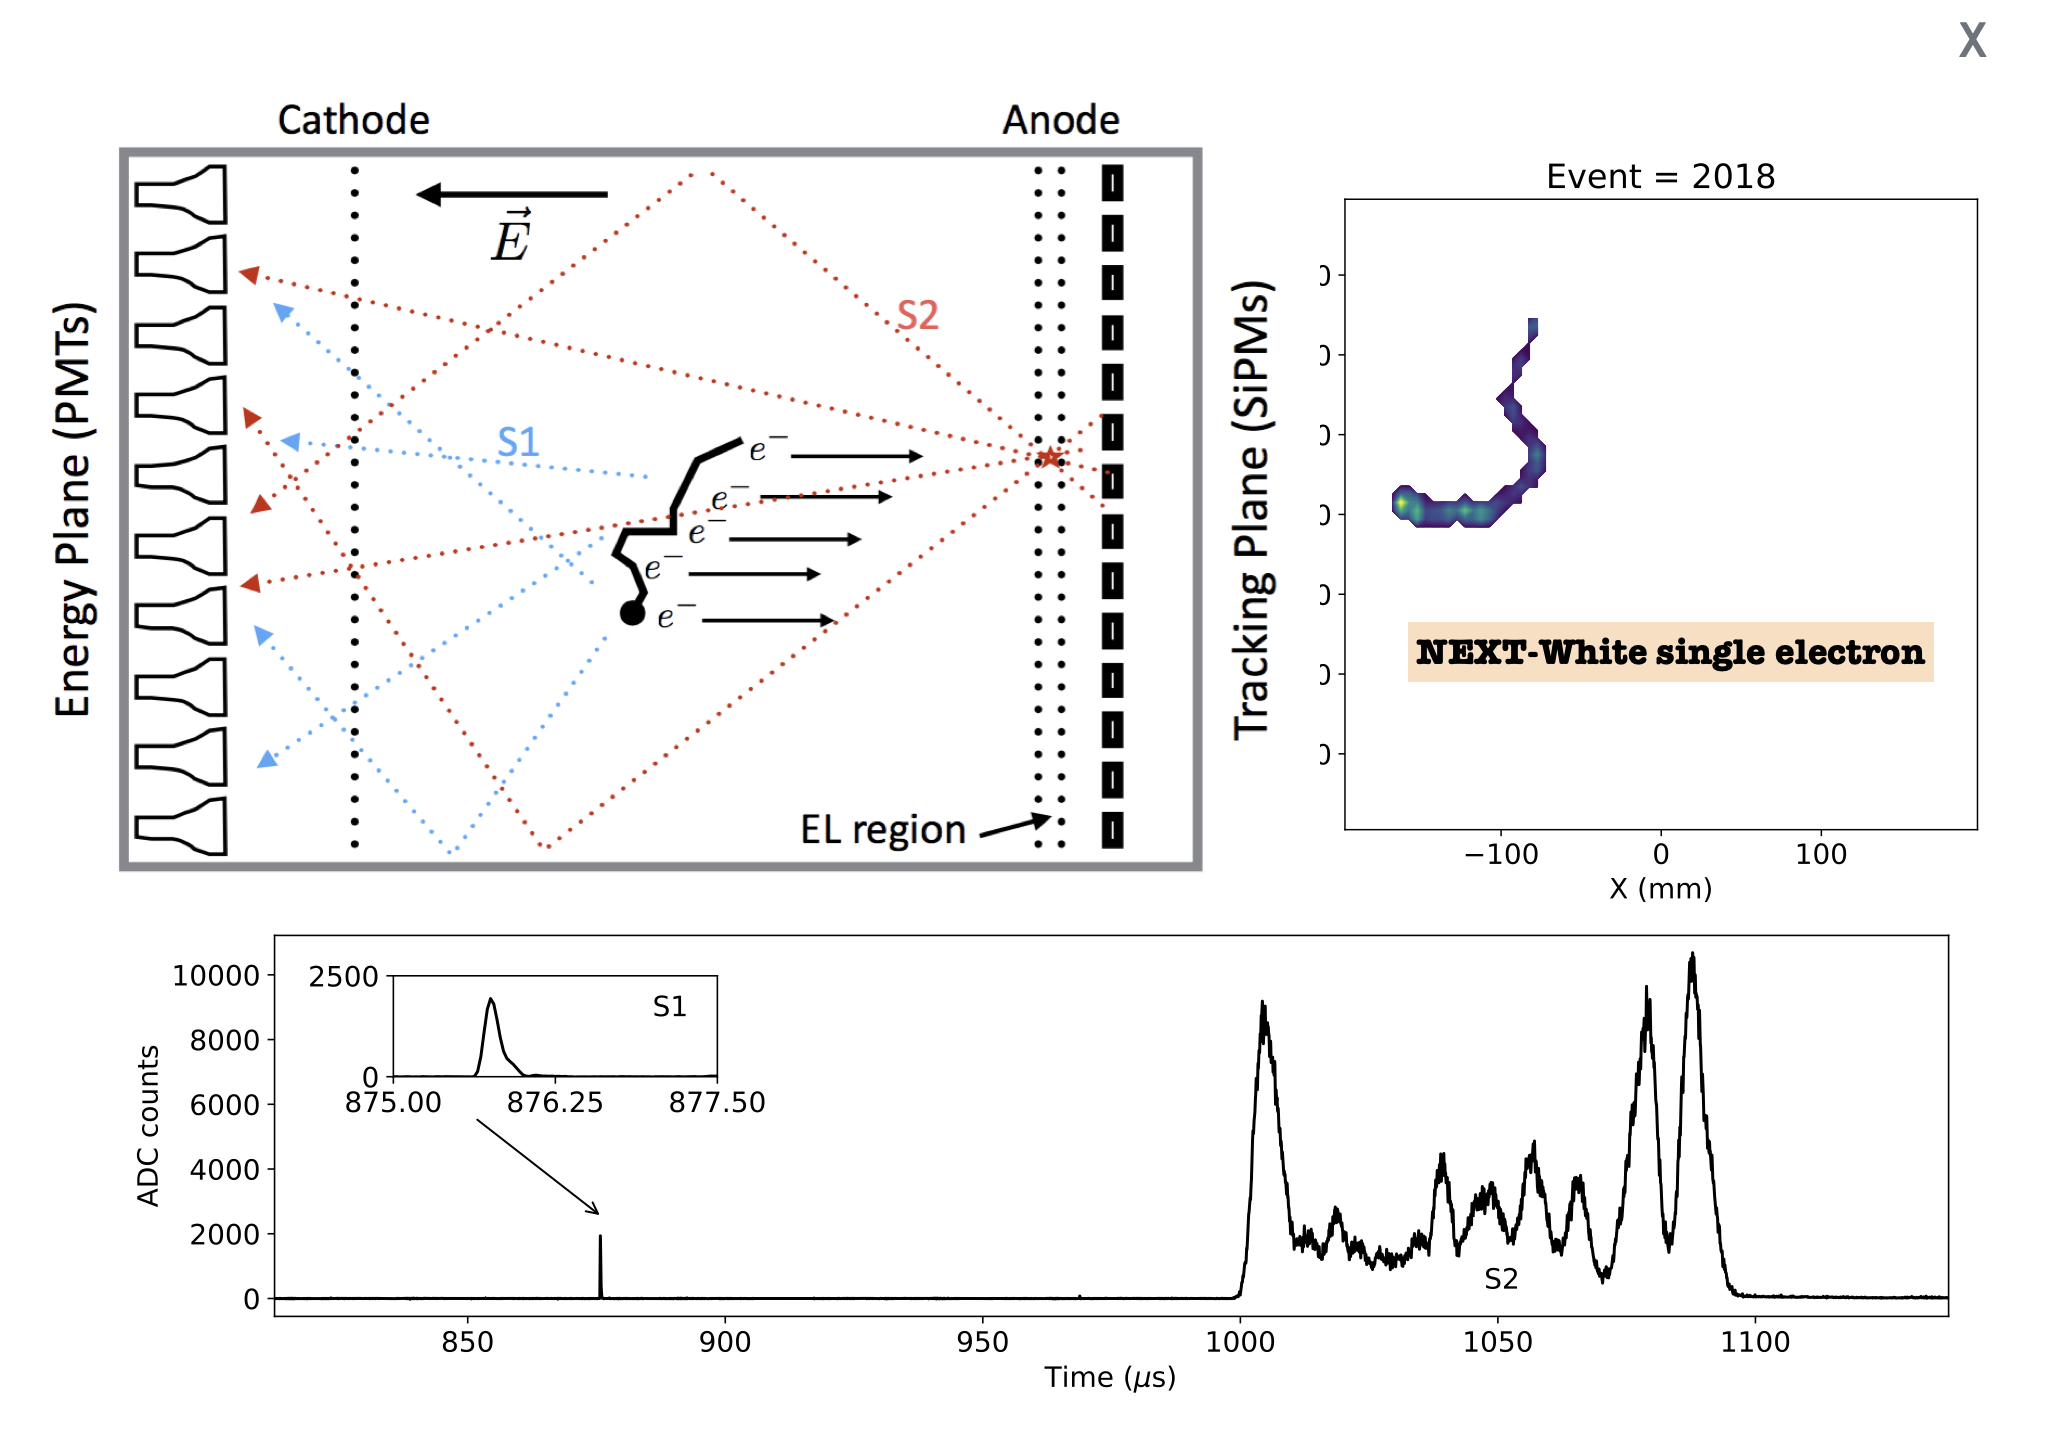
\includegraphics[scale=0.20]{nextpo.png}
%
% \column{0.50\textwidth}
%$\bullet~$ Primary scintillation \so\ signals the start-of-the-event, \tz.
%
%$\bullet~$ Secondary scintillation \st\  measures the energy of the event (energy plane, PMTs).
%
%$\bullet~$ Position in $z$ obtained from time difference between \so\ an \st. A measurement of \tz\ is essential to fiducialize the events and remove the large rate of background events that accumulate at the electrodes, and to correct for charge losses occurring during charge drift. Without such corrections, the performance of the detector both in terms of background rate and resolution is seriously compromised.
%
% $\bullet~$ Position in $x,y$ obtained from position and amplitudes of SiPMs (tracking plane).
% \end{columns}
%\end{frame}
%
%%%%%%%%
%
%\begin{frame}{S1 \& S2}
%
%$\bullet~$ In \XE\, the energy released in a \qbb\ event is 2458 keV. 
%
%$\bullet~$ This corresponds to $2458/76 = 32\ 342$~primary scintillation photons, distributed on a time of about 40 ns. Even with a modest light collection efficiency $\sim 1$\%, this result in a very clear signal, as in figures above.  
%
%$\bullet~$ The number of ionisation electrons is $2458/21.9 = 112\ 237$. Assuming that all those electrons are collected and amplified in the EL region, and assuming an EL gain of the order of 10$^3$, one gets $\sim 10^8$ EL photons. With a light collection efficiency of $\sim 1$\%, this result in about 10$^6$ photons, distributed over the length of the track.  
%
% $\bullet~$  The path length of the track depends on the gas pressure. In the case of a \bbonu\ event, one has two electrons with $\qbb = 2458 keV$, which move through the gas losing energy by ionisation and twisting around due to Coulomb MS. Eventually, they reach de Bragg Peak, near the end of their range and stop. The average path length (in z) at 10 bar is about 10 cm, which corresponds to about 100 $\mu$s, see figure.  
% \end{frame}
% %%%
% 
% \begin{frame}{Exercise 11}
% 
% $\bullet~$ Use Bette-Block equation for ionisation loss to estimate the path length of an electron with energy \qbb\ in gas xenon at 10 bar. BB formula is:
% \[
%\left( \frac{dE}{dx} \right) = K \cdot \frac{Z}{A} \cdot \frac{p}{p_0} \cdot \frac{1}{\beta^2} \cdot \left( \ln \left( \frac{2 m_e c^2 \beta^2 \gamma^2 T_{\text{max}}}{I^2} \right) - \beta^2 \right)
%\]
%
%Where:
%
%- \( K \): Constant factor (\(K \approx 0.307 \, \mathrm{MeV \, cm^2 / mol}\))
%
%- \( Z \): Atomic number of xenon (\(Z = 54\))
%
%- \( A \): Atomic mass of \XE\ (\(A \approx 137 \, \mathrm{g/mol}\))
%
%- \( p \): Pressure of the xenon gas w.r.t.  \( p_0 \) (reference pressure, usually 1 atm). 
%%- \( p_0 \): Reference pressure (usually 1 atm or 1 bar)
%%- \( \beta \): Velocity of the particle as a fraction of the speed of light (\(v/c\))
%%- \( \gamma \): Lorentz factor, \(\gamma = (1 - \beta^2)^{-1/2}\)
%%- \( m_e \): Mass of the electron (\(m_e c^2 \approx 0.511 \, \mathrm{MeV}\))
%
%- \( T_{\text{max}} \): Maximum kinetic energy that can be transferred to a free electron in a collision. 
%%approximately given by:
%%
%%  \[
%%  T_{\text{max}} = \frac{2 m_e c^2 \beta^2 \gamma^2}{1 + 2 \gamma m_e / M}
%%  \]
%  For MIPs,  \(T_{\text{max}} \approx 2 m_e c^2 \beta^2 \gamma^2\).
%  %, the mass of the projectile \(M\) is much greater than \(m_e\), simplifying \(T_{\text{max}} \approx 2 m_e c^2 \beta^2 \gamma^2\).
%
%- \( I \): Mean excitation energy of xenon (\(I \approx 482 \, \mathrm{eV}\))
%
%\end{frame}
%
%%%%
%\begin{frame}{Intrinsic energy resolution in xenon: Bolotnikov}
%\begin{columns}
%\column{0.40\textwidth}
%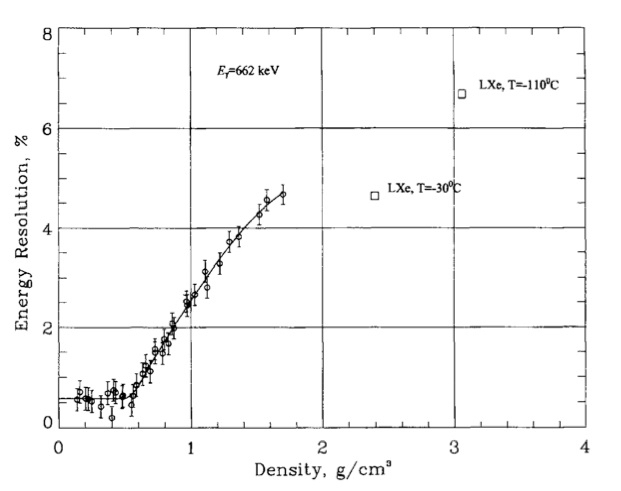
\includegraphics[scale=0.60]{energy-resolution-density.png}
%
% \column{0.60\textwidth}
%$\bullet$~As discussed in Lecture 1, excellent energy resolution is a crucial ingredient for a  \bbonu\ experiment. 
%
%$\bullet$~Figure (from Bolotnikov, 97) shows the energy resolution (FWHM)  for  662 keV gamma rays, as a function of xenon density, for the ionisation signal only.
%
%$\bullet$~ Observe the transition at density
%$\rho_t \sim 0.55{\mbox{g/cm}^3}$. Below this density, the energy resolution is approximately constant:
%$\delta E/E = 6 \times 10^{-3} {\rm ~FWHM}$. For densities greater than $\rho_t$, energy resolution deteriorates rapidly, approaching a plateau at LXe density.
%
%$\bullet$~ Extrapolating (as $1/\sqrt{E}$) to the \XE\ \qbb\ leads to
%$\delta E/E = 3 \times 10^{-3} {\rm ~FWHM}$.
%
%\end{columns}
%\end{frame}
%
%%%%
%
%\begin{frame}{Intrinsic energy resolution in xenon: GXe vs LXe}
%$\bullet$~ Bolotnikov experiment shows: a) that the intrinsic resolution that can be achieved in a GXe TPC at \qbb\ (measuring ionisation only) is very small (0.3 \% FWHM), and b) that measuring ionisation only yields a mediocre value of the energy resolution for a LXe TPC ($\sim 5$\% at 660 keV). 
%
%$\bullet$~This, in turn, implies: a) that a GXe TPC aiming to maximise energy resolution (a must for \bbonu\ experiments) must try to preserve the excellent energy resolution in gas, and b) that LXe TPC must do something else to improve their energy resolution (spoiler: measure primary scintillation and use the anticorrelation between ionisation and scintillation).  
%\end{frame}
%%%%%
%%For pure gaseous xenon (GXe)  various measurements \citep{Nygren:2007zz} show that
%%$F_{\rm GXe} = 0.15 \pm 0.02$.
%%\begin{equation}
%%	F_{GXe} = 0.15 \pm 0.02
%%\label{eq:gas-fano}
%%\end{equation}
%%
%\begin{frame}{Energy resolution in an EL TPC}
%%
%\begin{equation}
% R_E = 2.35 \, \, \sqrt{ \frac{F}{\bar{N}_e}
% + \frac{1}{\bar{N}_e} (\frac{J}{\bar{N}_{EL}}) + \frac{2}{\bar{N}_{ep}}}
% \label{eq:res}
% \end{equation}
%%
%
%$\bullet$~The first term in equation \ref{eq:res}, $R(Fano)$, correspond to the intrinsic resolution in xenon ($F_{\rm GXe} = 0.15 \pm 0.02$).
%
%$\bullet$~ The second term, $R(EL)$~to the resolution associated to fluctuations in
%electroluminescence production, and are described by the parameter $J = \sigma_{EL}^2/\bar{N}_{EL}$.
%
%$\bullet$~ The third, $R(EP)$~to fluctuations in the number of photoelectrons produced in the photosensor plane per \bbonu\ decay, $\bar{N}_{ep}$, which can be obtained as:
%$ \bar{N}_{ep} = k\ \bar{N}_e\ \bar{N}_{EL}$, 
%%
%where $k$~is the fraction of EL photons produced per \bbonu\ decay that gives rise to the production of a photoelectron. 
%
%$\bullet$~ {\bf Exercise 12}. Use equation \ref{eq:res} to estimate the expected resolution in a GPXe with EL amplification of 10$^3$ and light collection efficiency of 1\%.
%
%\end{frame}
%
%\begin{frame}{Energy resolution in an EL TPC}
%\begin{columns}
%\column{0.60\textwidth}
%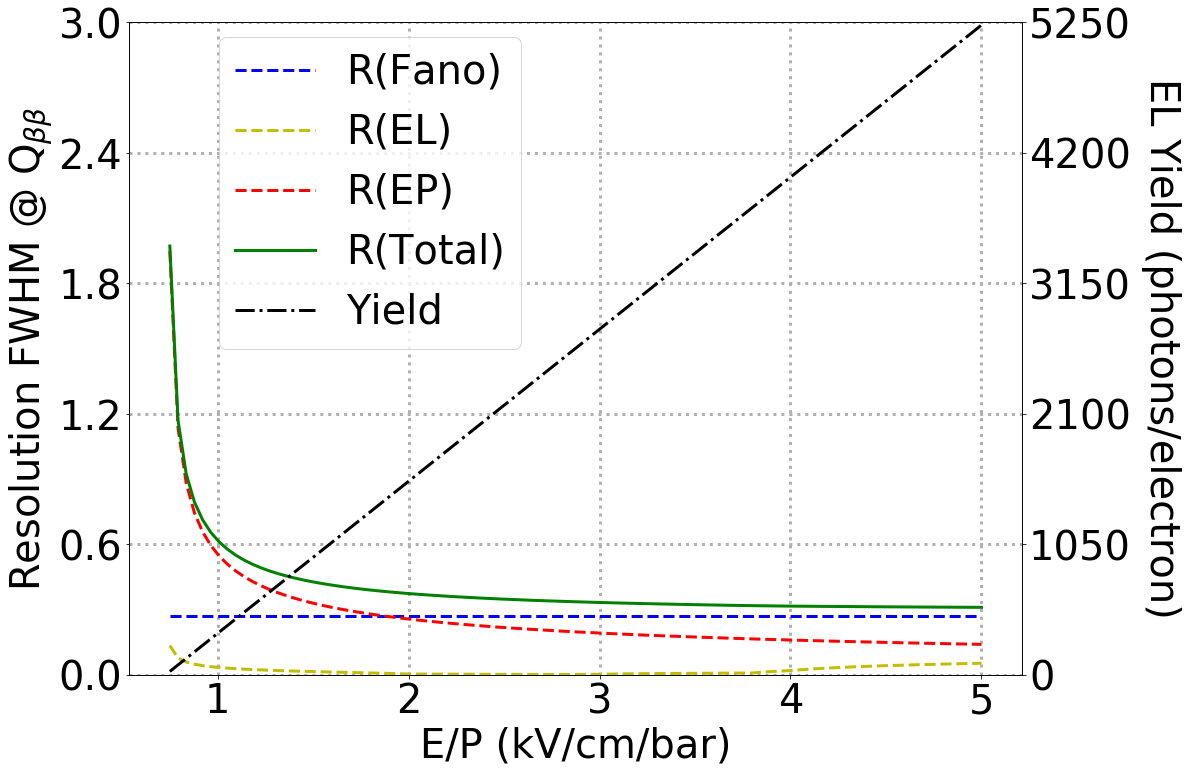
\includegraphics[scale=0.20]{resolution_15_bar.png}
%
% \column{0.40\textwidth}
%
%$\bullet$~Figure shows the EL yield and energy resolution, $R_E$ as a function of the reduced electric field of a HPXe EL TPC operating at 10 bar for the energy corresponding to \qbb. Notice that $R(Fano)$~is constant, $R(EL)$~is essentially negligible and $R(EP)$~improves quickly with the reduced field E/P. A typical value of operation for
%E/P is such that $R(Fano) = R(EL)$ ($E/P \sim 2$). The combined resolution at this value
%is around 0.5\% FWHM and the yield around $500$ photons per electron. Increasing $E/P$ results in very little resolution improvement.
%\end{columns}
%\end{frame}
%
%%%%
%
%\begin{frame}{Energy resolution in NEXT: DBDM}
%\begin{columns}
%\column{0.50\textwidth}
%\includegraphics[scale=0.10]{dbdm.png}
%%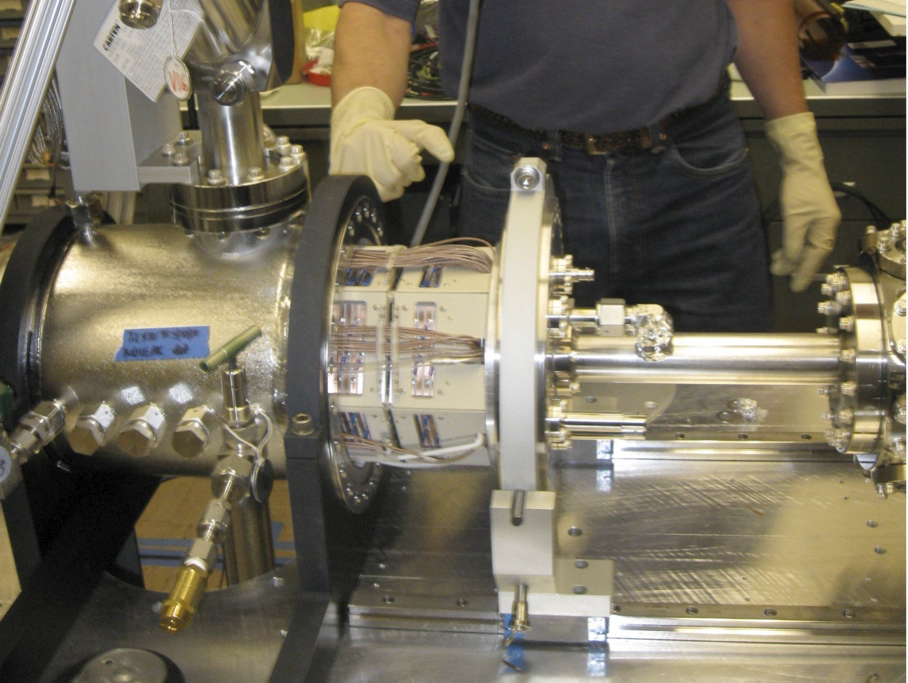
\includegraphics[scale=0.20]{dbdm_vessel.png}
%
% \column{0.40\textwidth}
%
%$\bullet$~The DBDM prototype at LBNL was the first NEXT prototype.  An array of 19
%photomultipliers (PMTs) measures \so\ primary scintillation light from the 8 cm long drift
%region and \st\ light produced in the 0.5 cm electroluminescence (EL) region 13.5 cm away
%from the PMTs. 
%\end{columns}
%\end{frame}
%
%%%%
%\begin{frame}{Energy resolution in NEXT: DBDM}
%\begin{columns}
%\column{0.50\textwidth}
%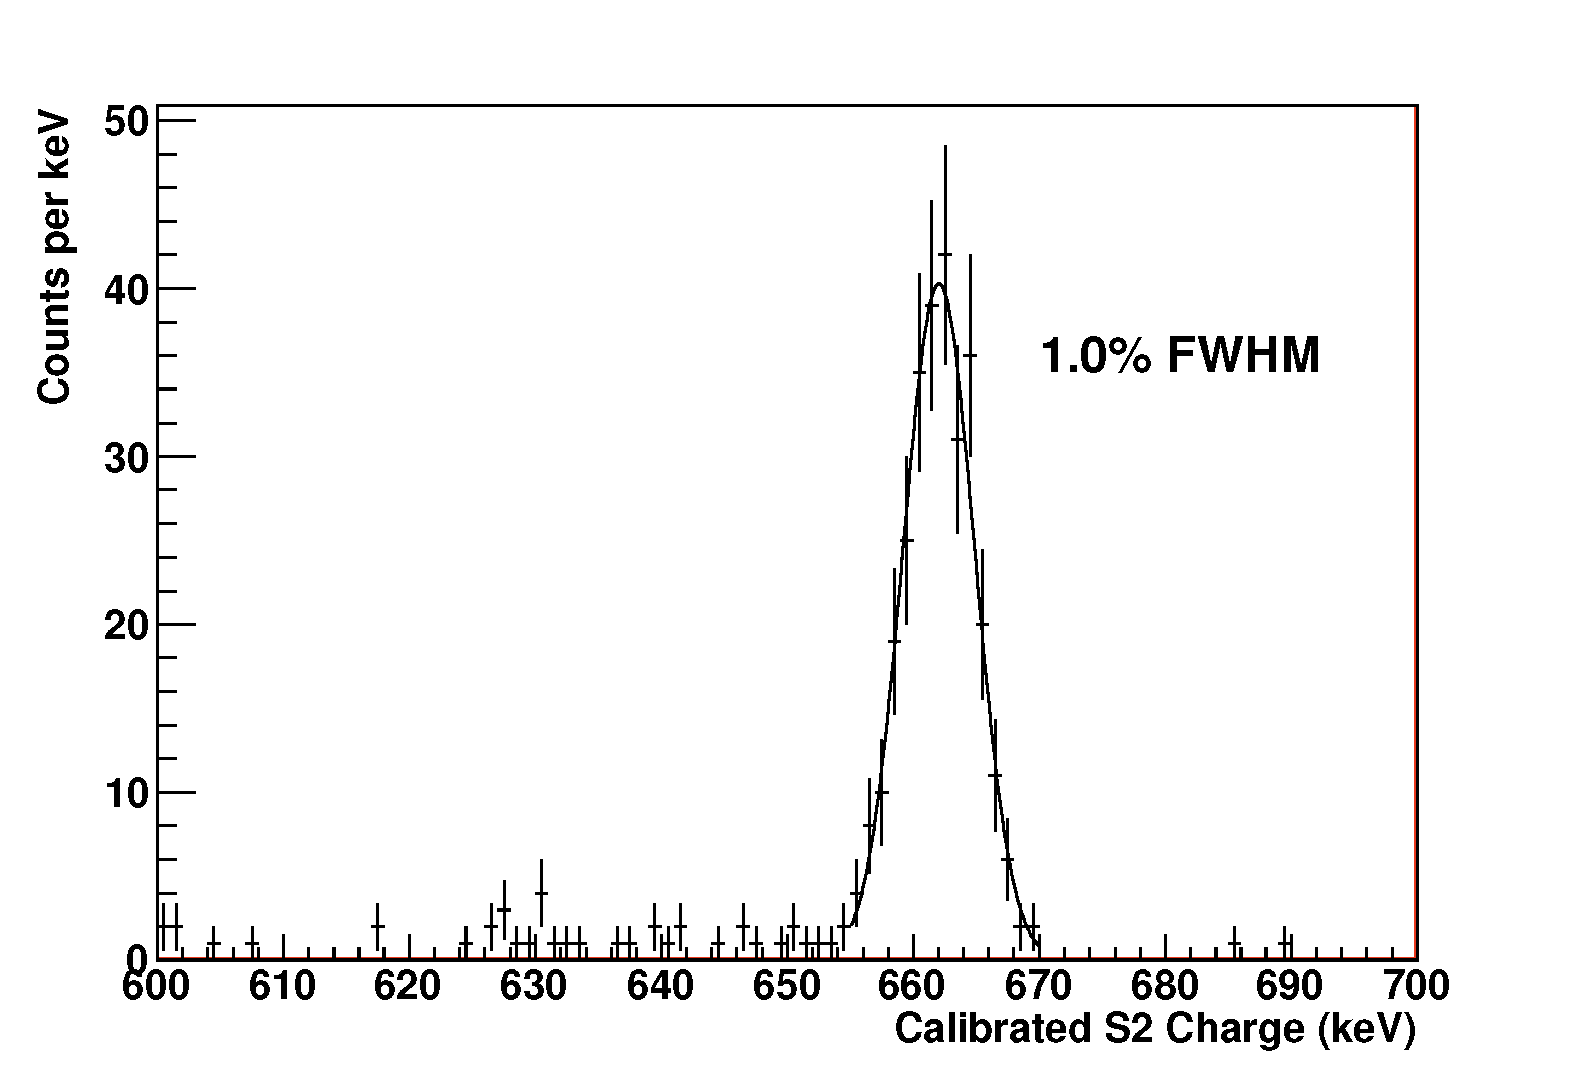
\includegraphics[scale=0.30]{dbdm_res.png}
%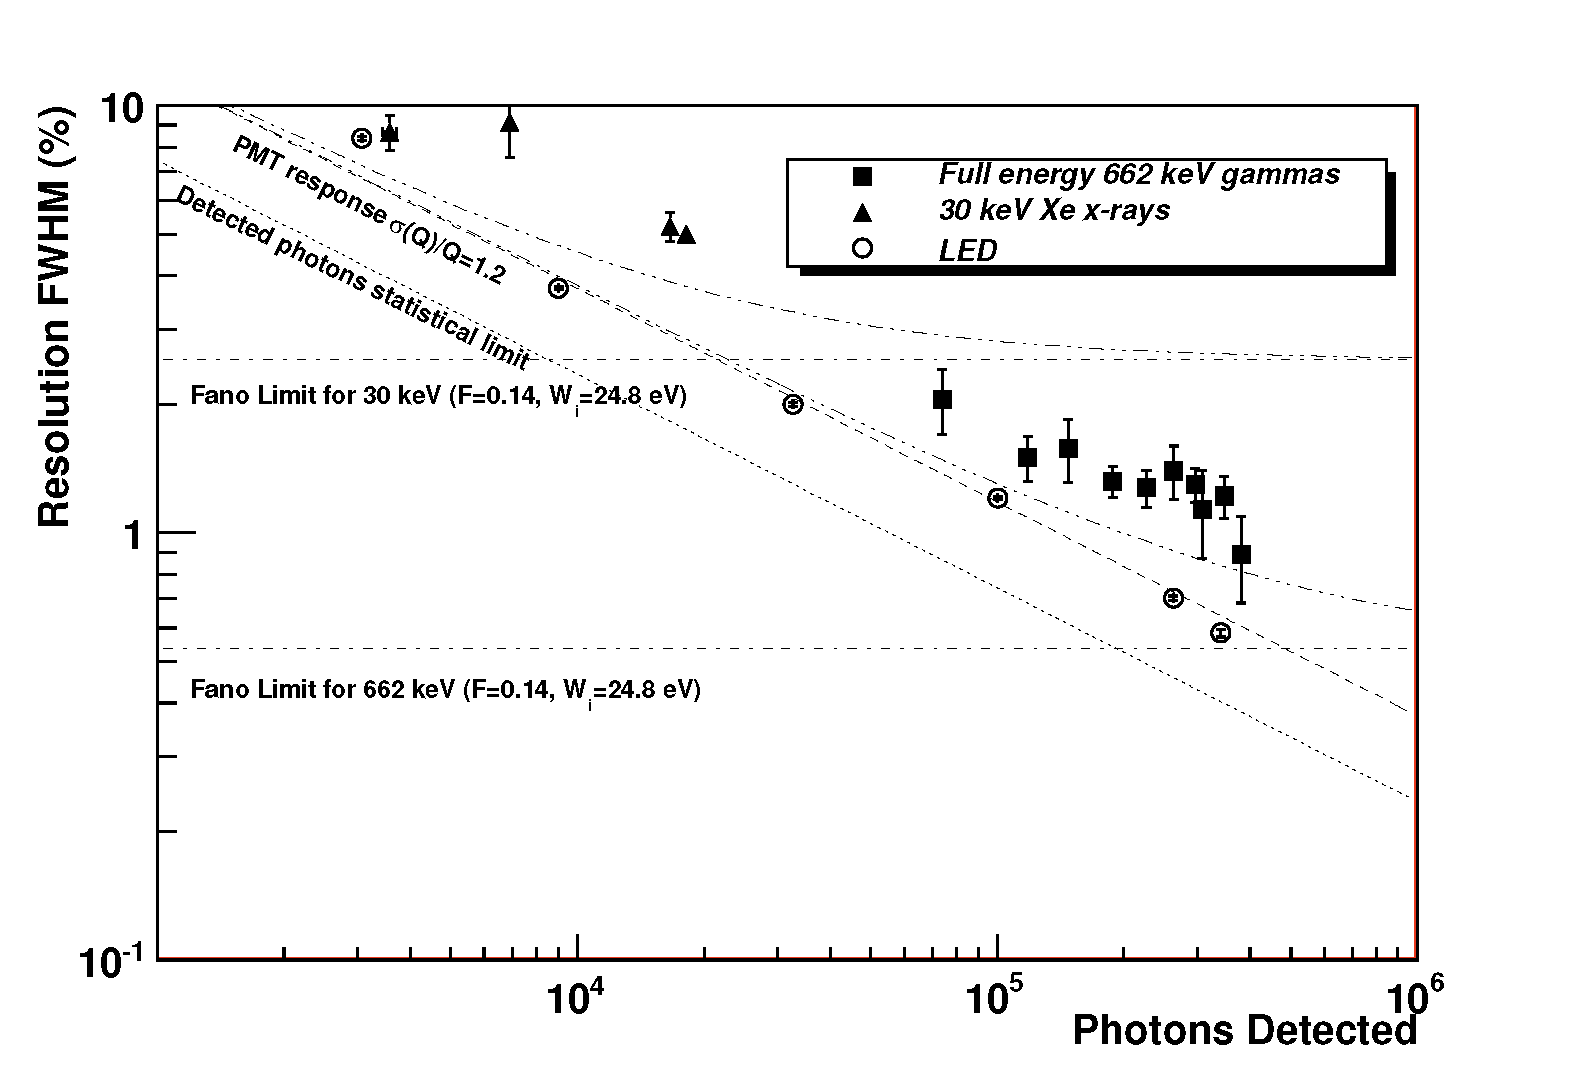
\includegraphics[scale=0.30]{dbdm_resolution.png}
%
% \column{0.50\textwidth}
%
%$\bullet$~DBDM measured an energy resolution of 1\% FWHM at 660 keV (15.1 bar), which scales up to 0.5\% FWHM at \qbb\, as predicted by analytical calculations.
%
%$\bullet$~ Data points show the energy resolution for gammas (squares) and xenon X-rays (circles), as 
%a function of the number of photoelectrons. The expected resolution is also shown. 
%\end{columns}
%\end{frame}
%
%
%%%%
%\begin{frame}{What about avalanche multiplication?}
%
%$\bullet$~Two problems: 1) the fluctuation in the gain, $G$, is considerably larger than $F$~in EL multiplication, and thus becomes the dominant term in the resolution. 2) electron multiplication in pure xenon is difficult, due to the fact that VUV scintillation light, copiously produced with the multiplication process, ejects electron from metallic surfaces defining the electrodes. Those electrons, in turn, ionise the gas to the point of breakdown.
%
%$\bullet$~The use of quenchers, on the other hand, suppresses the primary scintillation light. Without primary scintillation is not possible to define \tz\ and thus a fiducial volume cannot be well defined and the experiment becomes pray of backgrounds arising from the metal grids. ``Magic gases'', capable to absorb the VUV light emitted by xenon and re-emit it at a more manageable wavelength (e.g., in the visible region), without introducing extra fluctuations, have been sought, so far without success.
%
%\end{frame}
%
%\begin{frame}{Micropatterns devices}
%\begin{columns}
%\column{0.50\textwidth}
%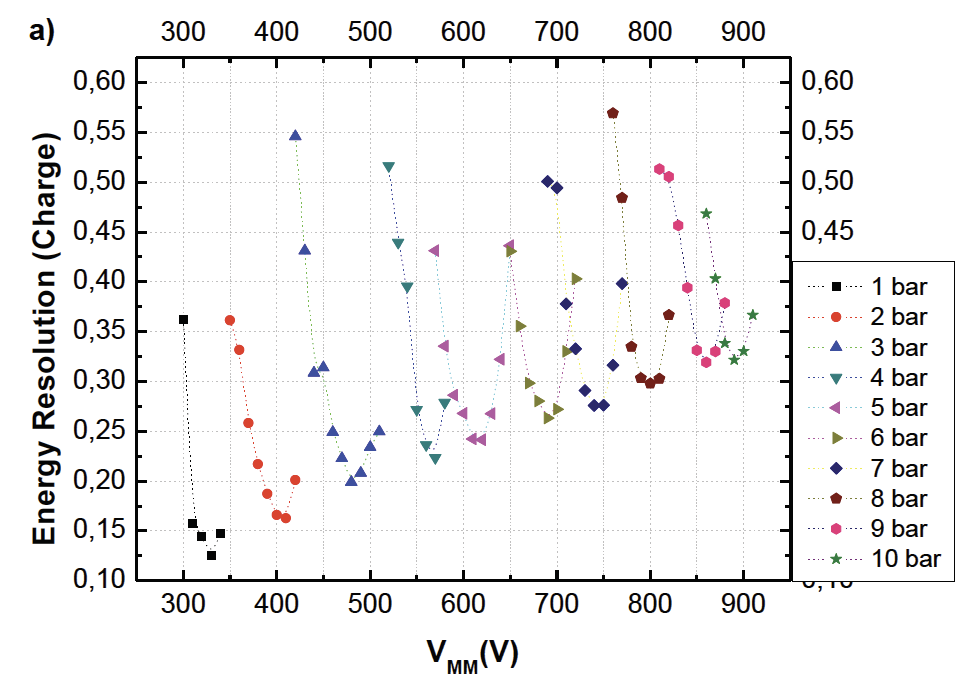
\includegraphics[scale=0.22]{MicromegasResolution.png}
%
%\column{0.50\textwidth}
%$\bullet$~Another possibility is to use micro-pattern devices, such as Micromegas  or GEMs whose confined geometrical structure makes them capable to operate at high pressure without quenchers.
%
%$\bullet$~This possibility was explored as a part of NEXT R\&D.
%While Micromegas were found, indeed,
%robust enough to allow operation in pure xenon and at high pressures, their resolution was measured to degrade with increased pressure. It was found that the resolution attainable at \qbb\ by  micro-bulk micromegas at 10 bar would be $3\%$, to be compared with that of $0.5\%$ found by DBDM. 
%\end{columns}
%\end{frame}
%
%
%%%%
%\begin{frame}{Diffusion}
%$\bullet$~As the ionisation electrons (and the positive ions) drift towards the anode (cathode) under the action of the electric field, they interact with the noble gas atoms, resulting in both longitudinal and transverse
%diffusion.
%
% 
%\end{frame}
%
%%%
\end{document}